\documentclass[12pt]{article}
\pdfpagewidth 8.5in
\pdfpageheight 11.0in
\usepackage{fullpage}
\usepackage{url}
\usepackage{graphicx}
\usepackage{subfigure}
\usepackage{booktabs}
\usepackage{multirow}
\usepackage{rotating}
\usepackage{float}
\usepackage{acronym}
\usepackage{setspace}
\usepackage{amsmath}
\usepackage[hypcap]{caption}
%\onehalfspacing
\usepackage{pdfpages}
\usepackage{tabularx}
\usepackage{bigstrut}
\usepackage{epstopdf}
\usepackage{hyperref}
\usepackage{caption}
%\usepackage{subcaption} is incompatible with subfigure
\usepackage{lscape}
\usepackage{longtable}
\usepackage[section]{placeins}

\title{CubeSat Deformable Mirror Demonstration\\Preliminary Design Review\\}
\author{Kristin L. Berry (KB)\\
Ashley K. Carlton (AC)\\
Zachary J. Casas (ZC)\\
James R. Clark (JC)\\
Vladimir V. Eremin (VE)\\ 
Zaira G. Garate (ZG)\\ 
Julian Lemus (JL)\\
Immanuel David Madukauwa-David (IM)\\
Tam Nguyen T. Nguyen (TN)\\
Alexandra E. Wassenberg (AW)\\\\\\\\\\
Department of Aeronautics and Astronautics\\
Massachusetts Institute of Technology\\
}

\date{\today}

\begin{document}
\maketitle
\newpage

\tableofcontents
\listoffigures
\listoftables


\section*{List of Acronyms}
\begin{acronym}

\acro{COTS}{Commercial Off The Shelf}
\acro{CG}{Center of Gravity}
\acro{DeMi}{Deformable Mirror Demonstration}
\acro{DM}{Deformable Mirror}
\acro{DOD}{Depth of Discharge}
\acro{EPS}{Electrical Power System}
\acro{FOV}{Field of View}
\acro{LEO}{Low-Earth Orbit}
\acro{MEMS}{Microelectromechanical Systems}
\acro{P-POD}{Poly-Picosatellite Orbital Deployer}
\acro{PDM}{Power Distribution Module}
\acro{PSF}{Point Spread Function}
\acro{ADCS}{Attitude Determination and Control System}
\acro{IMU}{Inertial Measurement Unit}
\acro{STK}{Satellite Tool Kit}

\end{acronym}
\newpage

%%%%%%%%%%%%%%%%%%%%%%%%%%%%%%%%%%%%%%%%%%%%%%%%%%%%%%
\section{Introduction - AW}

Deformable mirror wavefront control systems correct for aberrations in the wavefront to produce high contrast images.  This technology has been employed in ground telescope observation to counter wavefront distortions induced by Earth's atmosphere.  However, deformable mirrors have yet to be utilized on a space platform.  Such an implementation could remove aberrations in the wavefront due to speckles from diffraction, noise, phase errors, and thermal drift.  A proposed CubeSat Deformable Mirror demonstration (DeMi) will begin the process of testing adaptive optics technology in the space environment for future implementation on space telescopes and potentially free-space laser communication.  The use of deformable mirrors in conjunction with coronographs on-board space telescopes will be able to produce images with higher achievable contrast in the direct imaging of exoplanets.  This document presents a detailed overview of the role and design of the payload for the DeMi mission, a high actuator count MEMS deformable mirror yet to be tested in space, as well as the preliminary designs of the various satellite subsystems which support the flight of the payload in low Earth orbit.  

\subsection{Mission Statement}
The mission of the Deformable Mirror Demonstration is to provide a low-cost, quick-access platform on which to demonstrate microelectromechanical (MEMS) wavefront control deformable mirror imaging technology on-orbit.

\subsection{Motivation}
The driving force behind the DeMi mission is the desire to directly image Earth-like exoplanets in the search for signs of life, requiring imaging technology that can produce high contrast and dynamic range images.  However, current high-performance space telescope technology suffers from wavefront aberrations, such as speckles, which can result from diffraction, noise, phase errors, and thermal drift and reduce the achievable image contrast \cite{cahoy-unpublished}.

A solution to this problem is to implement adaptable wavefront control imaging technology in the form of a deformable mirror system. Specifically, a Boston Micromechanics
Mini MEMS Deformable Mirror \cite{bos-micro-demi}, shown in Figure~\ref{fig:Intro_demi} will be used. In the deformable mirror system, a wavefront sensor measures aberrations in an approaching wavefront. An adaptive optics computer then calculates the errors in the wavefront reflecting off of the deformable mirror surface by subtracting the wavefront from a reference wavefront \cite{adaptive-optics-overview}. Finally, electrostatic actuators in an array beneath the membrane surface of the mirror individually deform the surface to correct the wavefront. A comparison of the effects of a flat and deformable mirror on an aberrated wavefront is demonstrated in Figure~\ref{fig:Intro_wavefront}.   

\begin{figure}[!ht]
\centering
\includegraphics[width=2in]{images/introduction_1.png}
\caption{Boston Micromechanics MEMS Deformable Mirror \cite{bos-micro-demi}}
\label{fig:Intro_demi}
\end{figure}

\begin{figure}[!ht]
\centering
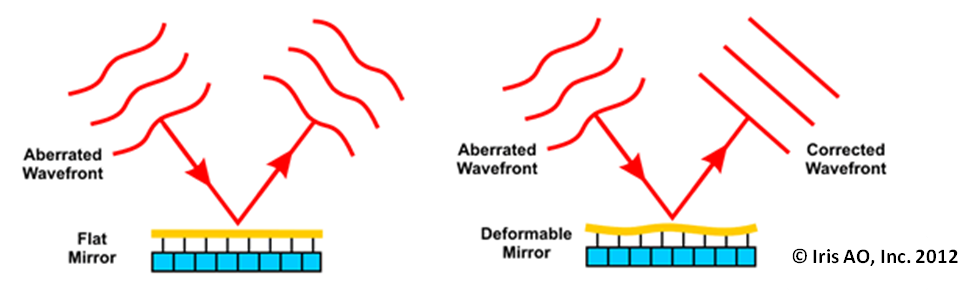
\includegraphics[width=4in]{images/introduction_2.png}
\caption{Comparison of the effects of a flat and deformable mirror on an aberrated wavefront}
\label{fig:Intro_wavefront}
\end{figure}

Adaptive optics technology is currently being used in conjunction with coronographs in ground telescopes to correct for distortions caused by Earth's atmosphere and to resolve light from nearby objects.  An example is seen in Figure~\ref{fig:Intro_exo} of three exoplanets imaged using the Palomar Observatory's Hale Telescope with adaptive optics technology \cite{serabyn2010}.

\begin{figure}[!ht]
\centering
\includegraphics[width=3.75in]{images/introduction_3.PNG}
\caption{Three exoplanets directly imaged using a combination of adaptive optics and a coronagraph with the Palomar Observatory's Hale Telescope.}
\label{fig:Intro_exo}
\end{figure}

However, factors such as high speeds of atmospheric turbulence and limited numbers of photons from targeted exoplanets reduce the achievable image contrast.  A solution to this issue is to incorporate deformable mirror wavefront control technology in high performance space telescope missions.  The DeMi mission will take the initial step by testing the stability, calibration, and predictability of a more complex, higher actuator count deformable mirror system in space.     

A space telescope utilizing a high performance coronograph and deformable mirror wavefront control system to directly image Earth-like exoplanets could potentially cost over a billion dollars.  Therefore, a 3U CubeSat platform was selected to conduct the DeMi mission.  The 3U CubeSat is a simple, standard platform, with low volume (10 cm x 10 cm x 30 cm) and mass (maximum 4 kg for a 3U CubeSat set by the CubeSat Design Specification document \cite{cubesat-specs}).   CubeSats additionally have low manufacturing and launch costs and can provide relatively quick and easy access to space, as opportunities exist for them to fly as auxiliary payloads on rockets for other planned missions. 

The technology that will be tested in the DeMi mission has a number of foreseeable future applications, including implementation on high performance space telescopes, such as for direct imaging of Earth-like exoplanets, or for use with free-space laser communication in order to correct for aberrations in the atmosphere \cite{cahoy-unpublished}.

\newpage
\section{Mission Overview - ZG}
		\subsection{Requirements}

		\paragraph{Mission Level Requirements}
		\begin{itemize}
				\item \textbf{MLR-1} The system design shall follow a 3-unit CubeSat platform.\\
				Parent Requirement: MS-1
				\item \textbf{MLR-2} The system shall primarily use commercial off the shelf (COTS) and CubeSat parts and components.\\
				Parent Requirement: MS-1
				\item \textbf{MLR-3} The system shall accommodate and operate a MEMS deformable mirror demonstration experimental payload.\\
				Parent Requirement: MS-1
				\item \textbf{MLR-4} The system shall operate and produce operational and experimental data for a period of $<$3 months$>$ [goal of 12 months].\\
				Parent Requirement: MS-1
		\end{itemize}

		\paragraph{Systems Requirements}

		\begin{itemize}
			\item \textbf{SYS-1} The system shall survive launch conditions.\\
			Parent Requirement: MLR-4
			\item \textbf{SYS-2} The system shall include electrical, mechanical, and software interfaces to the payload\\
			Parent Requirement: MLR-3
			\item \textbf{SYS-3} The system shall comply with the requirements and constraints listed in the most current CubeSat Design Specification (CDS) document \cite{mission_cubesat}. \\
			Parent Requirement: MLR-1
			\item \textbf{SYS-4} The system shall be capable of sending and receiving data and instructions to and from the ground.\\
			Parent Requirements: MLR-3, MLR-4
			\item \textbf{SYS-5} The system shall have a deorbit time of 25 years or less \cite{mission_deorbit}.\\
			Parent Requirement: MLR-4
		\end{itemize}

		\subsection{Design Overview}
		The DeMi mission will consist of one small satellite following the 3-unit CubeSat Design Specifications established by the California Polytechnic State University. The satellite will be the size of three stacked 10 cm cubes (called ``units''), measuring a total of 10 cm $\times$ 10 cm $\times$ 30 cm. In accordance to CubeSat specifications, the satellite's mass will not exceed 4 kilograms. In general, CubeSats are launched as secondary hosted payloads inside a standard Poly-PicoSatellite Orbital Deployer (P-POD) \cite{cubesat-specs}.
The CubeSat platform was selected because it offers a low-cost quick access option. Multiple vendors already sell many off-the-shelf CubeSat components with flight heritage for most standard satellite subsystems. Over the past several years, many university projects have been designed and flown on CubeSats. 


		\subsection{Concept of Operations}\label{sec:systems_conops}

		DeMi will be a 3-unit CubeSat on a Low-Earth Orbit (LEO) with an altitude of 500 km at an inclination of 40$^\circ$. This orbit inclination was selected in order to reach the NASA Wallops ground station located in the state of Virginia. The altitude of 500 km positions the satellite well within Low-Earth Orbit exposing the Payload to the space environment while still allowing 6 to 7 ground access opportunities per day for communications with the ground station. 

Figure~\ref{fig:Mission_ConOps} shows a timeline of the DeMi concept of operations and mission milestones. Immediately following separation from a standard P-POD, the satellite will begin to charge its primary batteries through solar panels covering the long faces of the structure. During this first stage, the satellite's antenna will be deployed and will emit intermittent beacon signals in order to be located by the ground station. The ADCS (Attitude Determination and Control System) torque coils will detumble the satellite and align it in a nadir-pointing position. The detumble stage will last approximately 2 weeks assuming a tip off rate of 10$^\circ$/sec. A detailed detumbling analysis can be found in Section~\ref{adcs_analysis}. The mission schedule allows up to one month for detumbling, yet any short delays during this stage would not be detrimental to the mission overall.


		\begin{figure}[!ht]
				\centering
				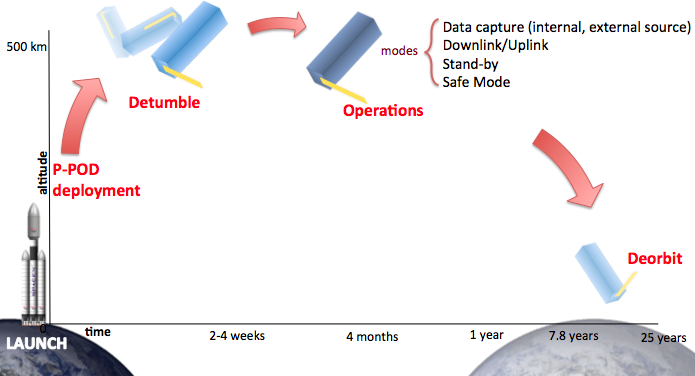
\includegraphics[width=5in]{images/MissionOverview_1.png}
				\caption{Timeline of the concept of operations for the DeMi Mission}
				\label{fig:Mission_ConOps}
			\end{figure}

		Once the satellite is in fully operational status, the Payload will begin to conduct scientific experiments and collect data. Two different data capture modes will be performed during the mission: internal source experiments will be done during the first 3 months of operations, while external source experiments will occur during the remainder of the mission. The satellite will attempt to downlink the collected data whenever it passes over the NASA Wallops ground station and is given instructions to begin downlink.  

The majority of the time, the satellite will be in stand-by mode; in other words, it will not be capturing or downlinking data. In case of a subsystem malfunction, the satellite will go into safe mode to diagnose the source of the problem. 

Given the satellite's altitude, inclination, and surface area, analyses performed using STK predict that the satellite will deorbit within 7.8 years. This timeline agrees with the current 25-year deorbit requirement outlined by NASA standards \cite{nasa-deorbit}.


\subsection{$N^2$ Diagram}

		The N$^2$ diagram was an essential tool in the early stages of the design process. It allowed the design team to determine the levels of interaction between different subsystems and exchange input and output variables and values. 

		\begin{figure}[!ht]
				\centering
				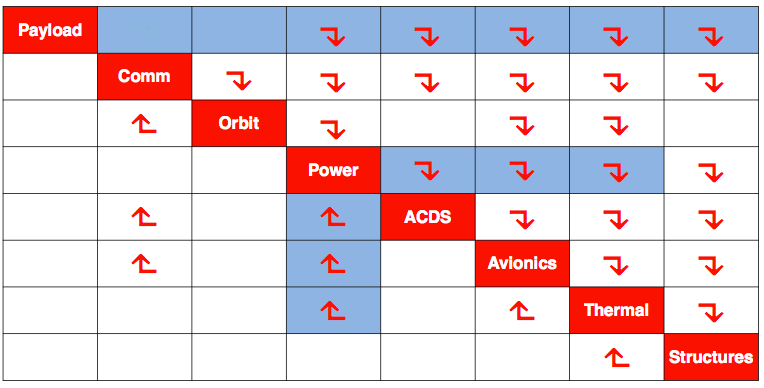
\includegraphics[width=5in]{images/MissionOverview_2.png}
				\caption{High-Level $N^2$ diagram showing input/output relationships between subsystems}
				\label{fig:Mission_N2}
			\end{figure}

		As highlighted Figure~\ref{fig:Mission_N2}, the Payload requirements drive the design of all the other subsystems. While the Payload does not receive design inputs from other subsystems, its design outputs cascade down effectively driving the design of the rest of the satellite. A more detailed view of the DeMi N$^2$ diagram can be found in Appendix 1.

	\subsection{System Level Budgets}
		\subsubsection{Mass}
		In agreement with CubeSat standards, the total mass of the satellite must not exceed 4 kg. Figure~\ref{fig:Mission_mass2} shows the total mass of the satellite broken down by subsystem. As of PDR, the design is projected to weight 3.26 kg and 3.90 kg with added margin. Following industry standards, the subsystem margin percentages used in this analysis correspond to the Mass Growth Allowance values for Preliminary Design published by the American Institute of Aeronautics and Astronautics \cite{mission_aiaa}. Figure~\ref{fig:Mission_mass2} illustrates that the mass of the satellite is driven primarily by the Payload, which takes up approximately one third of the total. The Power and ADCS subsystems closely follow with 26\% and 22\% respectively. 

			\begin{figure}[!ht]
				\centering
				\includegraphics[width=5in]{images/MissionOverview_3.png}

				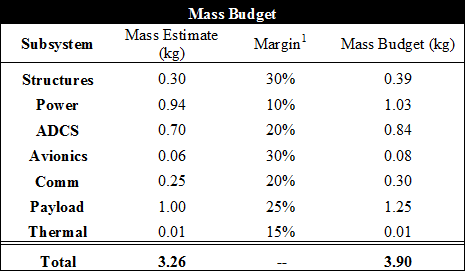
\includegraphics[width=5in]{images/MissionOverview_5.png}
				\caption{System Mass Budget}
				\label{fig:Mission_mass2}
			\end{figure}

		\subsubsection{Power}
		This section presents the power used by the spacecraft during each of its modes of operation as well as the power supplied by the solar panels and battery. 

The power used by the satellite during each mode is outlined in Figure~\ref{fig:Mission_power2}. The first two items, ``Safe/Uplink'' and ``Detumbling'', do not occur on a regular daily basis during the operational lifetime of the satellite, which is why their duration is not expressed in minutes per day and their values are not included in the average power calculation. 

During its operational period, the satellite will cycle between the data capture, downlink, and stand by modes. As shown in Figure~\ref{fig:Mission_power2}, the most power is drawn by the antenna in the Communications subsystem during downlink. 

The satellite is expected to require an average of 3.54 Watts with up to 4.18 Watts with an 18\% margin applied. This allowance percentage of 18\% was derived from input from course faculty and the fact that most components will be commercial off the shelf (COTS) with flight heritage. 

Curerntly, the Power system design carries a tight margin. The solar panels and battery are projected to supply up to 3.84 Watts; however, this would not satisfy the average power with margin needed at this stage in the design process. The power supplied is only 8.5\% higher than the expected power needed without margin. This issue is discussed in detail in Section~\ref{sec:power}.


			\begin{figure}[!ht]
				\centering
				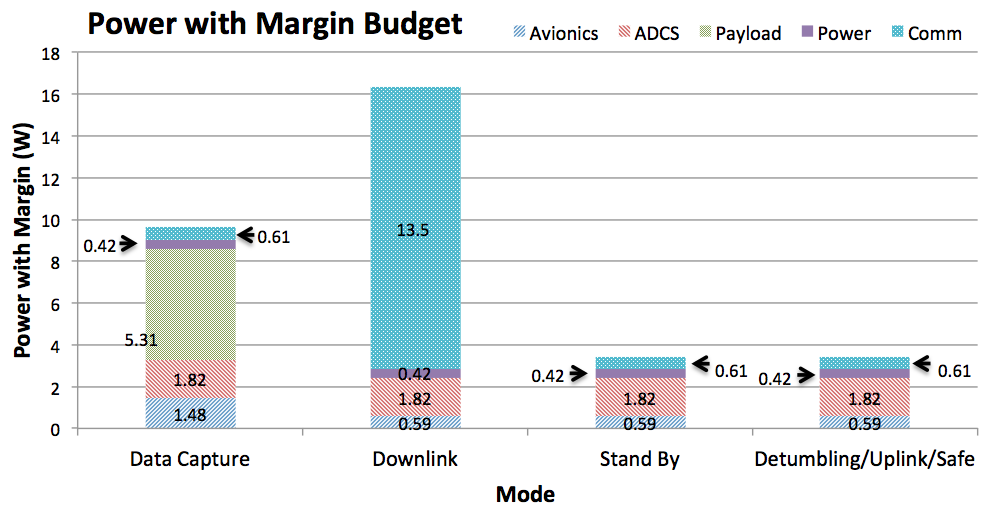
\includegraphics[width=5in]{images/MissionOverview_4.png}

				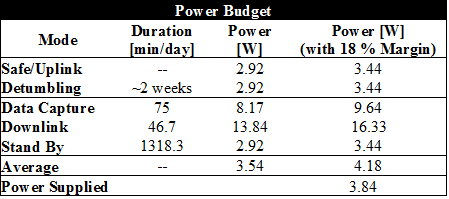
\includegraphics[width=5in]{images/MissionOverview_6.png}
				\caption{System Power Budget}
				\label{fig:Mission_power2}
			\end{figure}
\newpage			
\section{Subsystems}

\FloatBarrier
%%%%%%%%%%%%%%%%%%%%%%%%%%%%%%%%%%%%%%%%%%%%%%%%%%%%%%
% PAYLOAD

		\subsection{Payload}
The Payload for DeMi is an optical system that allows for the testing
and technology demonstration of a deformable mirror system.  It must include the following  elements: the deformable mirrors the
mission aims to test, a light source to create a wavefront, and a detector to measure the wavefront.  These components are attached
to an optical breadboard and are in an enclosure to block out external
light.  The challenge in this project is to create an optical system capable of testing the accuracy of current deformable mirror technology and evaluate its future applications while meeting the mass, volume and other constraints imposed by the 3U CubeSat platform.
			
\subsubsection{Requirements - AC}\label{sec:payload_requirements}

\begin{itemize}
\item \textbf{PLD-1} The Payload shall command a MEMS deformable mirror to run a pre-defined test sequence for at least 5 minutes each orbit. \\ 
Parent Requirements: MLR-3, MLR-4
\item \textbf{PLD-1.1} The Payload shall have the ability to control any combination of actuators within 0.001 s of each other, at a minimum rate of 100 Hz, with a minimum stroke of 1.5  $\mu$m, and with a precision of at least 1 nm.\\
Parent Requirement: PLD-1
\item \textbf{PLD-2} The Payload shall have the ability to measure and reconstruct the optical wavefront at one wavelength for the duration of a 5 minute test sequence each orbit at a frequency of at least 10 Hz.\\
Parent Requirements: MLR-3, MLR-4
\item \textbf{PLD-2.1} The Payload shall have the ability to measure the optical wavefront at a minimum rate of 10 Hz for at least one minute each orbit.\\
Parent Requirement: PLD-2
\item \textbf{PLD-2.2} The Payload shall have the ability to measure the optical wavefront at a minimum rate of 100 Hz for at least 30 seconds each orbit.\\
Parent Requirement: PLD-2
\item \textbf{PLD-2.3} The Payload shall have the ability to reconstruct the optical wavefront with a minimum accuracy of 100 nm rms.\\
Parent Requirement: PLD-2
\end{itemize}

There are two types of requirements on the Payload.  The first set (PLD-1) applies to the features of the deformable mirror system.  The second set (PLD-2) pertains to the measurement and reconstruction of the wavefront.  The complete requirements document can be found in Appendix~\ref{app:requirements}. 

The requirements on measuring and reconstructing the wavefront (PLD-2) apply to the detector.  Nominally, the detector must operate (capture images) for at least 5 minutes per orbit, and be able to function at a minimum of 10 Hz (PLD-2). The requirement is further separated into a ``Diagnostic Mode'' used for calibration and full frame images, and a ``Burst Mode'', used for data capture.  In ``Diagnostic Mode'', the Payload is required to take images for at least a minute per orbit at 10 Hz (PLD-2.1).  In ``Burst Mode'', the Payload is required to take images for at least 30 seconds per orbit a minimum of 100 Hz (PLD-2.2).  For both modes, the reconstruction accuracy must be a maximum of 100 nm rms (PLD-2.3).
			
			\subsubsection{Decisions Made and Trade Studies - AC, KB}

\paragraph{Payload Architecture - AC}

While in future applications the deformable mirror system will be used to aid
in observing stars or other objects, the mission goal of DeMi is to characterize the deformable 
mirror system, and to accomplish this with commercial off the shelf (COTS) components
whenever possible, providing a quick and simple platform for space (MLR-3, MLR-4).
As mentioned previously, there are a few key components that are integral to the design: the 
deformable mirror system to test, a light source to create a wavefront, and a detector to measure the wavefront.
To keep the design as simple as possible, the use of an internal light source, such as a laser, is  desirable for the technology demonstration. 

Many techniques exist for measuring and reconstructing a wavefront \cite{FGadaptiveoptics}.  These can be divided into sensored and sensorless approaches.
Sensorless approaches, such as the Gerchberg-Saxton-Based Estimation Scheme \cite{gerchberg}, are likely to be used for a direct imaging application of a large space telescope mission for their ability to eliminate non-common path optical errors.  However, sensorless approaches require additional computational resources, time, and occasionally additional detectors or detector translation \cite{cahoy2013}.  
Therefore, only sensored
approaches are considered for this platform due to the compact form
factor, the desire to use simple COTS components, and processing capabilities. There are numerous wavefront
sensing approaches that could be implemented, as well as
modified versions of those presented here, but the two designs discussed are chosen for their ability to be simply implemented in a compact platform.
While other designs (see Section~\ref{sec:payload_interferometer}) may be able to achieve higher precision, the Shack-Hartmann wavefront sensing system fits in the allotted volume with minor modifications to components, and allows for sufficient mirror characterization, meeting our mission goal and requirements (Section~\ref{sec:payload_requirements}). Therefore, the Shack-Hartmann wavefront sensing design in Figure~\ref{fig:SHWFS} has been chosen to image the wavefront.

\subparagraph{Design Decision: Shack-Hartmann Wavefront Sensor - AC}

For the wavefront sensing design in Figure~\ref{fig:SHWFS}, a Shack-Hartmann lenslet array is used, allowing for accurate wavefront measurement and reconstruction sensitivity. The design has an internal source (laser diode), whose path is denoted by a dotted red line, and an aperture for imaging an external source, whose path is denoted by a dotted green line.

\begin{figure}[ht]
\centering
  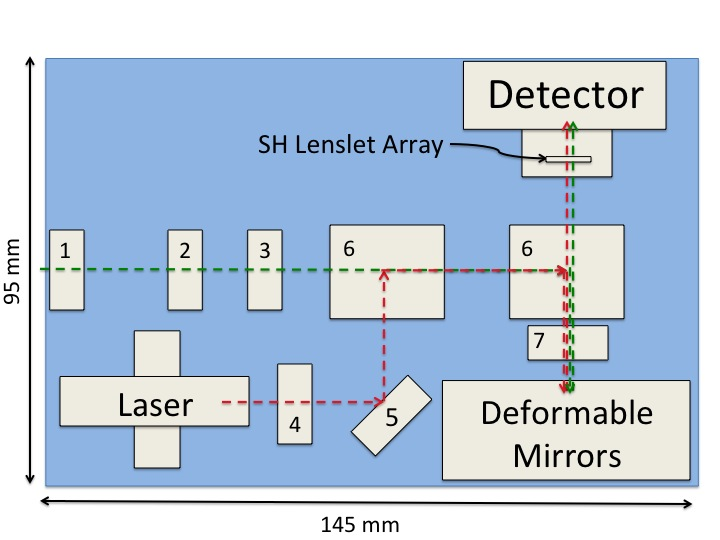
\includegraphics[width=5in]{images/payload_SHWFS.jpg}
\caption{Design decision: Wavefront Sensing design with a Shack-Hartmann lenslet array}
\label{fig:SHWFS}
\end{figure}

For the internal source, the laser diode module emits a collimated elliptical beam. This beam enters a linear polarizer (where its intensity is halved). The beam then encounters a flat mirror at 45 degrees, reflecting the beam 90 degrees, and proceeds to a primary beam splitter. Here, the beam is reflected 90 degrees to a secondary polarizing beamsplitter, and reflected another 90 degrees. The beam then goes through a quarter waveplate (where the beam is now elliptically polarized) before striking the deformable mirrors. The deformable mirrors reflect the beam back through the quarter waveplate, rendering the beam now linearly polarized with an orientation that allows it to pass through the secondary beam splitter. The beam then proceeds through the lenslet array, creating a spot diagram on the detector corresponding to shape of the wavefront (see Section~\ref{sec:payload_sh}).

For the external source, the wavefront beam enters a plano-convex lens and passes through a collimating lens. The beam then enters a linear polarizer (where the intensity is halved). The beam passes through the primary beam splitter, and then to the secondary polarizing beamsplitter, which reflects the beam 90 degrees towards the quarter waveplate and the deformable mirrors, as mentioned previously, and follows an identical path as the internal light source to the detector.

The chosen design allows the detector to image both an internal and external source. While the mission goal can be accomplished with just an internal source, the ultimate goal of using this technology on a larger space telescope for imaging of bright stars motivates the use of an external source. Therefore, the option for an external source is included in the design.

Due to the added complexity required of the ADCS system on a CubeSat platform, the external source imaging will not require a precise star acquisition and navigation system. In contrast, with pointing knowledge from ADCS, the shutter on the aperture will be commanded open when a bright star is in the field of view (FOV). The maximum slew rate for imaging the external source is discussed in Paragraph~\ref{sec:pointing_requirement}.  Based on preliminary models looking at five bright stars (Alpha Centauri, Arcturis, Canopus, Sirius, and Vega), the satellite would expect to see the same bright star every orbit for an average of three to five minutes\footnote{Based on an STK simulation performed by Annie Marinan.}.  The pointing requirement on the maximum ADCS slew rate to keep the star on the same pixel on the detector is discussed in Section~\ref{sec:pointing_requirement}.

It is necessary that the aperture for imaging an external source be small, given the volume constraints of the CubeSat platform after accommodating all of the key elements of the system (deformable mirror, mirror driver electronics, detector, and necessary imaging optics). Due to the physical size of these key elements, it is not practical to design the external source imaging as a typical reflecting telescope. While it may be possible to accommodate an aperture lens with relatively large diameter ($>60$ mm), the corresponding longer focal length would not fit in the volume, and the space for resizing the beam is limited. While the smaller aperture will limit the angular resolution and sensitivity and increase the size of the point spread function (PSF), tight angular resolution is not a requirement for this technology demonstration. Therefore, this design has an aperture lens with diameter 12.7 mm, with a minimum focal length on the order of its diameter. Using the Rayleigh criterion, the angular resolution (width of the center of the PSF) at 500 nm is 9.907".

The current design allows for open and closed loop control.  Images and centroid solutions can be sent to the ground, allowing for evaluation of the mirror performance over time.  In addition, closed loop control (active correction of the wavefront on orbit) can also be implemented on board using the centroids and calculated slopes to command the mirrors.  Calculating mirror response from slopes requires little additional processing \cite{centroids}. 

All optical elements of the system are preliminarily chosen.
(See Appendix~\ref{app:payload_components} for the full list of
elements with part numbers and mass totals.)  Glass elements are
chosen to be UV fused silica over other glasses whenever possible for
their better performance in space \cite{radiation_optics} due to a
high coefficient of thermal expansion and better UV transmission.  All
elements also have anti-reflective coatings that are efficient in the
visible spectrum (400 - 700 nm).  All components in Figure~\ref{fig:SHWFS} are shown with their mounts.  However, the mass and volume of the mounts are only estimates of the custom mounts that will be built for all optics.  Custom mounts will be built to adapt the optics for space applications.  All elements must be mounted in stress-free mounts (e.g., no glass touching metal) and mounted to an optical breadboard with multi-footed lens tubes that are made of aluminum, or of a metal that has a similar coefficients of thermal expansion as the lens it holds.  Future modeling and optimization of the optical design will yield more exact component choices.

\subparagraph{Other Designs Considered: Michelson Interferometer with Nanopositioner - AC}\label{sec:payload_interferometer}
The interferometer design shown in Figure~\ref{fig:interferometer} is slightly modified from a typical interferometer due to volume constraints on the Payload and the requirement for high contrast imaging. It has an internal source (laser diode), whose path is denoted by a dotted red line.
The laser beam is first resized, passes through a neutral density filter, then is reflected 90 degrees by a
flat mirror. The light is then divided by a beam splitter oriented 45
degrees to the beam. The transmitted beam travels to the deformable
mirror where it is reflected back towards the beam splitter. Half of
the beam is deflected by 90 degrees at the beam splitter and strikes
the detector. The reflected beam travels to the flat mirror on the
nanopositioner where it is reflected and half of it then is transmitted
through the beam splitter and reaches the detector. The two beams that
reach the detector interfere to produce fringes \cite{traeger} that are analytically well understood as a function of beam coherence/divergence and mirror tip/tilt \cite{demtroeder} and that can be simulated for a variety of different deformable mirror shapes.

\begin{figure}[ht]
\centering
  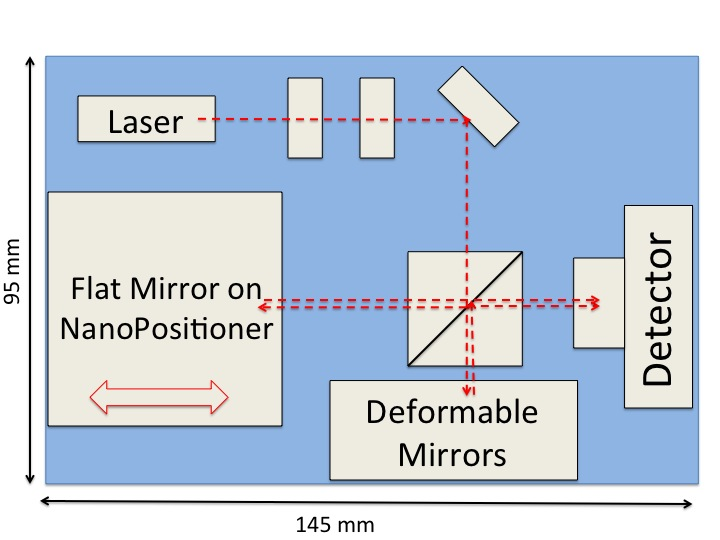
\includegraphics[width=5in]{images/payload_interferometer.jpg}
\caption{Other considered design: Michelson Interferometer with the flat mirror on a nanopositioner.}
\label{fig:interferometer}
\end{figure}

For this particular design, as mentioned previously, a flat mirror is on a nanopositioner, or a piezo linear stage, which moves in increments of fractions of the incoming wavelength. This allows for higher precision fringe patterns, allowing for better mirror characterization.

What is not shown in Figure~\ref{fig:interferometer} is the controller for the nanopositioner \cite{newport_nanopositioner}. It does not currently fit within the constraints of the satellite in terms of mass, volume, and power needs, and would require significant modifications, if it were to be implemented. Also, the additional moving part (nanopositioner) increases the risk and complexity of the mission, making the Shack-Hartmann wavefront sensor the design choice.

\subparagraph{Payload Operations - AC}
For the initial demonstration and on-orbit testing, an internal light
source will be used. This eliminates any Payload specific requirements
on the satellite's attitude and inclination. For the latter half of
the mission, an external light source will be used, in order to attempt to image the optical wavefront from a star.  All downlinked files will be timestamped.

\begin{enumerate}
\item{\textbf{Status Checks}}
After detumbling, and two weeks of commissioning, as described in
Section~\ref{sec:systems_conops}, the Payload will perform a status check of all instruments. This includes the deformable mirror system, the detector, and the laser. Each element will be turned on and checked for error or status codes. Any available status information directly from the deformable mirrors, detector, and laser will be sent to the ground.

\item{\textbf{Calibration}}
The next phase is to calibrate the system using the ``Diagnostic Mode" requirements outlined in Section~\ref{sec:payload_requirements}.  This involves turning on the laser and recording several images in this configuration with the detector, without deforming the mirrors (acts as a flat mirror). From these images, on-board processing algorithms can find the centroids \cite{centroids} and average them to obtain new `standard centroids', which will be used for wavefront comparison calculations throughout the remainder of the mission. These images, averages, and new centroid solutions will be sent to the ground and stored on-board.

\item{\textbf{Data Capture: Internal Source}}
The next, and most important, stage is data capture using the internal source. The laser is turned on, then the mirror is deformed by a predetermined test sequence of commands, and the wavefront is imaged on the detector. The test sequence will include `poking' one actuator at a time, and `poking' combinations of actuators in commonly known shapes, such as Zernike polynomials and Fourier modes.  Then, the images are read from the detector, centroids are found, and one full image and the collection of centroid solutions are sent down to the ground and stored on-board.  Local wavefront slopes will be found from the centroid solutions using simple on-board algorithms, and the mirrors will be commanded for active wavefront correction on-board.

\item{\textbf{Data Capture: External Source}}
The second part of data capture will be with an external source. This external source will be a bright star, such as Vega or Sirius, as mentioned previously.  With
knowledge from ADCS, the shutter will be commanded open, and the laser
will be commanded off, allowing an external source to be imaged. The
images will be read from the detector, the centroids found, and one
full frame image along with the collection of centroid solutions will be
sent to the ground and stored on-board.  Identical to data capture with an internal source, local wavefront slopes will be found from the centroid solutions using simple on-board algorithms, and the mirrors will be commanded for active wavefront correction on-board. 

\end{enumerate}

\paragraph{Deformable Mirror System - KB} \label{par:payload_dms}
%I should probably write a general introduction to DMs, huh? 
There are only two vendors which sell commercial off-the-self options for MEMS deformable mirrors that will fit inside a CubeSat: Boston Micromachines, and Iris Adaptive Optics. These options are summarized in Table~\ref{table:payload_dms}. The Boston Micromachines Mini DM comes in three different sizes of stroke and aperture. Stroke referes to the maximum amount the mirror can 'push' a segment outward, and the aperture is simply the aperture of the DM. Since there is little room for resizing optics in our system, the aperture of the DM
acts as a stop. As such, larger apertures are strictly better for the accuracy of the wavefront we can reconstruct. While the Iris AO PT111 does have a larger aperture \emph{and} a larger stroke, which are both
better for accuracy, its driver board is larger and much more difficult to modify than the BMC Mini's. As such, we selected the largest BMC mini DM, with a 2.25 mm aperture and a stroke of 5.5 $\mu \text{m}$.

\begin{table}[!ht]
  \caption{Deformable Mirrors Considered for Payload Design}
    \begin{tabular}{|l||l|llll|}
      \hline
     &Requirement&BMC Mini 1.5 $\mu$m& Mini 3.5 $\mu$m & Mini 5.5 $\mu$m &Iris AO PT111 \\ \hline
    Stroke& Min 1.5 $\mu$m & 1.5 $\mu$m & 3.5 $\mu$m & 5.5 $\mu$m & 5 or 8 $\mu$m \\ \hline
    Rate& Min 100 Hz& 8 kHz & 8 kHz & 8 kHz & $>$ 6.5 kHz\\ \hline
    Control Precision& 1 nm & 0.09 nm& 0.2 nm & 0.3 nm & 0.3 or 0.5 nm \\ \hline
    Response Time& 0.001 sec & 20 $\mu$s & 100 $\mu$s & 500 $\mu$s& $< 200 \mu$s \\ \hline
    Aperture& - & 1.5 mm & 2.0 mm &2.25 mm&3.5 mm\\
      \hline
    \end{tabular}\label{table:payload_dms}
\end{table}

\paragraph{Detector - KB} \label{par:payload_detector}
%.. and a general introduction to detectors. 
For a detector, we chose the UI52-41LE-M CMOS detector from
IDS. Critically, it has a 5.2$\mu m$ pixel size, which is smaller than
the pixel sizes we looked at for the alternatives. Since accuracy is a
function of pixel size, maximizing pixels per subaperture is very
important. Alternatives we considered included the DCC1545M and the
e2v CCD47-20 frame transfer CCD (Table~\ref{table:payload_detectors}). 

\begin{table}[!ht]
  \caption{Detectors Considered for Payload Design}
    \begin{tabular}{|l||l|llll|}
    \hline
    Detector                      & Req. PLD-2
    &47-20&DCC1545M&UI1221LE-M&UI5241LE-M\\ \hline \hline
    Manufacturer&-&e2v&Thorlabs&IDS&IDS\\ \hline
    Type&-&Frame transfer CCD&CMOS&CMOS&CMOS\\ \hline
    Full frame rate&  10 Hz            & 5 MHz                       & 25 fps                 & 87.2 fps            & 50 fps              \\ \hline
    Subframe rate& 100 Hz            & -                           & 79 fps                 & 100 fps             & 102 fps             \\ \hline
    Accuracy       & 100 nm rms        & 11.2 nm rms                 & 45 nm rms              & 45 nm rms           & 45 nm rms           \\ \hline
    Data Rate& -                 & 52.4 Tbit/sec               & 259 Mbit/sec           & 207 Mbit/sec        & 310 Mbit/sec        \\\hline
    \end{tabular}\label{table:payload_detectors}
\end{table}


\paragraph{Shack-Hartmann Lenslet Array - AC} \label{sec:payload_sh}

A Shack-Hartmann lenslet array consists of a matrix of small lenses (called lenslets) of the same focal length, where the array is focused on the detector. Each lenslet forms a “spot”, creating a spot diagram on the detector. Figure~\ref{fig:lenslet_array} demonstrates incoming light through a lenslet array. The local tilt of the wavefront across each lenslet can then be calculated from the position of the focal spot on the sensor; the displacement, $\Delta x$, equals the local slope of the wavefront. Any phase aberration can be approximated to a set of discrete tilts. By sampling an array of lenslets, all of these tilts can be measured and the whole wavefront approximated. Only tilts are measured, so the lenslet array cannot detect discontinuous steps in the wavefront.

\begin{figure}[ht]
\centering
  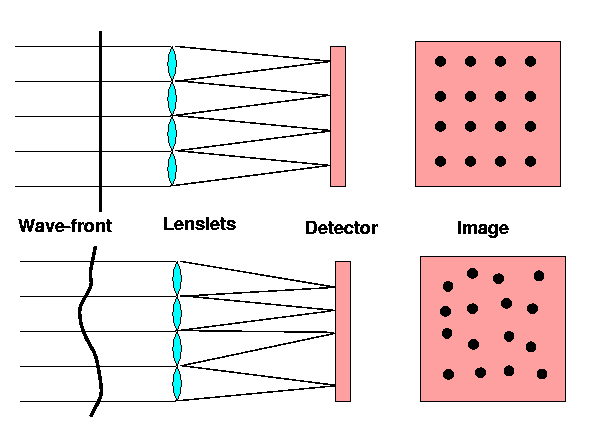
\includegraphics[width=5in]{images/payload_SH.png}
\caption{The result of two wavefronts, plane (top)
  and abberated (bottom), entering a Shack-Hartmann lenslet array, and their
  resulting spot diagrams on the detector \cite{ctio_AO}.}
\label{fig:lenslet_array}
\end{figure}

To get the best measurement of the wavefront, the maximum number of spots, and therefore lenslets, is desired. As a result, for a constant beam size, a lenslet array should be chosen with the lowest pitch (distance from the center of each lens) in order to get the maximum number of spots for the beam. 

Therefore, the microlens array MLA150 was chosen from ThorLabs \cite{MLA150} (see Figure~\ref{fig:MLA150}), with a pitch of 150 $\mu$m.
The lenslet is 10 mm square, so it contains about 66 by 66 lenslets. It is mounted in the lens tube on the detector. For an approximate beam size of 2.25 mm (see Paragraph~\ref{par:payload_dms}), approximately 15 by 15 lenslets will be used of the lenslet array.  See Section~\ref{sec:payload_pixels} for a discussion of the pixels used on the detector per lenslet.

\begin{figure}[ht]
\centering
  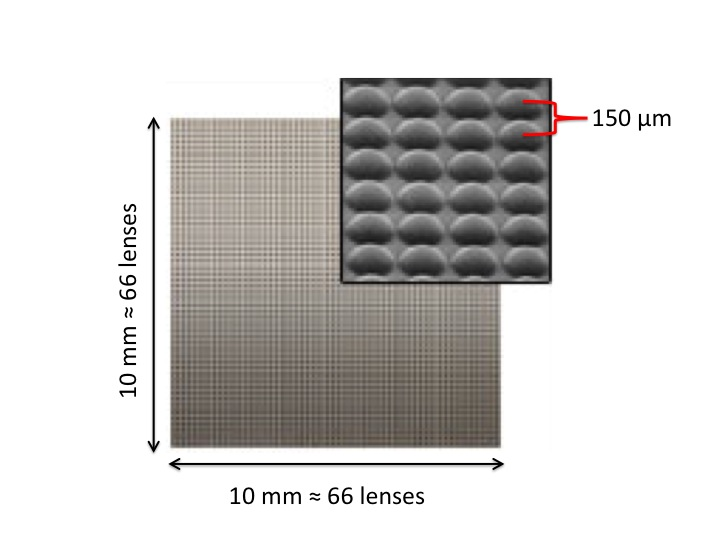
\includegraphics[width=4in]{images/payload_MLA.jpg}
\caption{The MLA150 lenslet array from ThorLabs \cite{MLA150} chosen for the Shack-Hartmann Wavefront Sensing design consists of many microlenses, aligned closely together.}
\label{fig:MLA150}
\end{figure}

\paragraph{Pointing Requirement - KB}\label{sec:pointing_requirement}

To determine the pointing requirement, we first need to calculate the plate scale of the detector.
%and the amount of time needed to get a reasonable SNR for a star of a reasonable magnitude. 
The plate scale of the detector is the relationship between angular distance on the sky and pixel size on the detector, and is typically measured in arcseconds per pixel.  
%%% (INSERT MATH) 

$\text{maximum slew rate} = \frac{\text{plate scale}}{\text{minimum exposure time}}$
%is there a better way to do simple formulas that don't really need to be in equation form? 

\paragraph{Data Rates to Avionics - KB}

The rate at which payload will output data to avionics is a function of the number of pixels of the image selected for output (either the full frame or a subframe,) the number of bits per pixel, and the rate at which images are taken in frames per second (fps.) The formula is simply: $r_{out} = \text{pixels} \times \frac{\text{bits}}{\text{pixel}} \times \text{fps}$
%is there a better way to do simple formulas that don't really need to be in equation form? 
These values and the calculated data output rate for our selected detector is shown in Table~\ref{table:payload-data-rates}. Note that the 640 x 480 subframe is the mode we will use for ``Burst Mode,'' and the 1280 x 1024 full-frame will be used for ``Diagnostic Mode.'' Each meets their respective requirements. 

\begin{table}
\begin{center}
\caption{Data output rates by detector and subframe mode}
\begin{tabular}{|c||c|c|} 
\hline
& Fullframe & Subframe \\
\hline
IDS CMOS UI5241LE-M  &  &   \\
\hline
Bits Per Pixel &  10 & 10\\
Pixel Resolution  & 1280 x 1024 & 640 x 480 \\
Image rate &  50 fps & 102 fps\\
Data Rate & 655.4 Mbit/sec & 310 Mbit/sec \\
\hline
\end{tabular}\label{table:payload-data-rates}
\end{center}
\end{table}

\paragraph{Shack-Hartmann Lenslet Array - AC}
			
\subparagraph{Pixels per Lenslet Spot}\label{sec:payload_pixels}
In order to image the spots created by the Shack-Hartmann microlenslet array, spots must fall on their own unique pixels.  At least four pixels are required per lenslet spot (a two by two square of pixels) to account for the event in which a spot lands between two pixels, or at the center of four pixels.
The incoming beam is 2.25 mm (Paragraph~\ref{par:payload_detector}).  This corresponds to about 15 by 15 spots. The detector has a pixel size of 5.2 $\mu$m, so a 2.25 mm beam corresponds to about 425 px square.  Therefore, over twenty pixels are available for each lenslet spot, so there is no concern for multiple spots falling on the same pixel. 
				
				\subparagraph{Actuators per Lens}
The chosen BMC deformable mirrors have a total of 32 actuators (a 6 by 6 array, with no corners) with an actuator pitch of 450 $\mu$m \cite{BMC}.  The Shack-Hartmann lenslets have a pitch of 150 $\mu$m, so there will be a minimum of four spots devoted to each actuator.  Therefore, there is no concern for individual actuators to be untested or characterized properly.

			\subsubsection{Summary of Outputs - AC}

The Payload's operational requirements are major drivers for the design of the rest of the satellite. A summary of mass totals, power needs, and thermal requirements of all major Payload components can be found in Table~\ref{fig:payload_summary_table}.  
During data capture mode, the Payload must be kept within $0^\circ$C to $50^\circ$C, will draw a maximum power of 4.5 W, will output a maximum data rate of 550 Mbit/s, and, during external data acquisition only, has a maximum slew rate of 4.7'/s. 
With all components, the Payload is 1.00 g, and 1.25 kg with a 25\% margin.  

\begin{table}
\caption{Summary of the mass totals, power needs, and thermal needs of the major Payload components.}
\begin{tabular}{|c||c|c|c|c|} \hline
	\textbf{Component} & \textbf{Mass (g)} & \textbf{Power (W)} & \textbf{Thermal, operating ($^\circ$C)} & \textbf{Thermal, storage ($^\circ$C)} \\ \hline \hline
Laser diode & 24.45 & 0.0045 & -10 to 50 & unknown \\
Detector & 46.64 & $<$ 2 W & 0 to 50 & -20 to 80 \\
DMs + Driver & 189.9 & $<$ 2.5 W & -10 to 50 & unknown \\
Optical Breadboard & $\sim$250 & -- & -- & -- \\
Optical Enclosure & $\sim$300 & -- & -- & -- \\ \hline \hline
Totals & 996.9 & 4.5 max & 0 to 50 & -20 to 80 \\ \hline
\end{tabular}\label{fig:payload_summary_table}
\end{table}

\subsubsection{Risks - KB}


			\subsubsection{Future Work - AC}

Future work includes optical modeling of the system using the software ZEMAX \cite{zemax}. Modeling the system with ZEMAX will determine the
  final beam profile on the detector.  This will allow for more precise calculations of data rates, for example.  Optimization of the space will
  be determined to find the best choice of components.  Thermal
  effects on the beam and optical components will be also analyzed, along with the effects of slight misalignments (i.e. with lenslet array).

Also, to determine the feasibility of the interferometer with the nanopositioner design, discussions with various nanopositioner manufacturers are needed to resolve if the nanopositioner elements can be appropriately modified for a CubeSat platform.  Preliminarily, a nanopositioner would require additional power and processing.  Further effects on other subsystems needs to be determined. 

Furthermore, while the design allows for imaging of an external source, when and how to image an external
  source still needs to be determined. Specific bright stars need to be chosen, and their revisit times calculated more precisely based on the orbital parameters unique to DeMi.

Lastly, specific properties of the deformable mirror system need to be explored.  For example, a stroke analysis needs to be performed.  Also, research needs to be done to try to predict the deformable mirror system's performance in a space environment, and how this might be quantified and corrected.

\newpage
\FloatBarrier
%%%%%%%%%%%%%%%%%%%%%%%%%%%%%%%%%%%%%%%%%%%%%%%%%%%%%%
% POWER
			
		\subsection{Power - JC} \label{sec:power}
			\subsubsection{Requirements}
			
			\begin{itemize}
				\item \textbf{POW-1}  Power subsystem shall supply 3.54 watts (calculated in Equation~\ref{eq:power-required}) to power bus on average over each orbit.
				\\
				Parent Requirement: MLR-3
				\item \textbf{POW-1.1}  Power subsystem shall have solar panels to supply power to other systems while satellite is in sunlight and recharge batteries for eclipse.
				\\
				Parent Requirement: POW-1
				\item \textbf{POW-1.1.1}  Solar panels shall supply 3.54 watts after 12 months of operation.
				\\
				Parent Requirement: POW-1.1
				\item \textbf{POW-1.2}  Power subsystem shall have rechargeable (secondary) batteries to supply power during eclipse.
				\\
				Parent Requirement: POW-1
				\item \textbf{POW-1.2.1}  Secondary batteries shall have 6.5 watt-hours of capacity (calculated in Equation~\ref{eq:power-batt-size}) after 12 months / 6,000 cycles (calculated in Equation~\ref{eq:power-num-cycles}).
				\\
				Parent Requirement: POW-1.2
				\item \textbf{POW-2}  Power subsystem shall supply 13.84 watts of power for peak operations
				\\
				Parent Requirement: MLR-3
			\end{itemize}
			
			\subsubsection{Decisions Made}
			
			The chosen solar panel configuration is four body-mounted side panels.  Body-mounted panels were chosen over deployable panels because they minimized the surface area of the satellite, which minimized the disturbance torques, and they are symmetrical, reducing the pointing constraints on the ADCS.  The zenith and nadir faces are left bare so that they can be coated with a paint that improves the thermal characteristics of the satellite.  The zenith face is also left bare to accommodate an aperture that will allow the payload to image external light sources; the limitations imposed by the placement of the aperture and the required shape of a top-mounted solar panel limit the available area for solar panels, making it impractical to panel.

The remainder of the power system is composed of a stack of modules to manage power distribution throughout the satellite.  An EPS (Electrical Power System) takes power from the solar panels and manages the current and voltage levels to ensure that the panels deliver power at maximum efficiency.  A secondary (rechargeable) battery supplies the satellite with energy during eclipse; the 10-watt-hour model was chosen, as this satisfies the required capacity and depth-of-discharge (see Equation \ref{eq:power-batt-size}).  A PDM (Power Distribution Module) supplies power to systems which are not part of the main system stack, such as the torque coils.

The satellite's power subsystem does not include a primary battery.  A primary battery was never included in the design because the satellite is covered on most sides by solar panels and is power-positive in detumbling mode, so it will charge as soon as it exits the P-POD.  The only reference to a Cubesat containing a primary battery was a description of a Cubesat that lacked solar panels entirely.\cite{libertad-1}

\subsubsection{Trade Studies}
			
			STK was used to compare the average power obtained by the solar panels under several circumstances.  The two variables were the inclusion or omission of a solar panel on the top face of the satellite, in addition to the four side-mounted panels, and the orientation of the satellite in its orbit.  The three orientations considered were ``face-first'', ``corner-first'', and spinning about its long axis.  The face-first and corner-first attitudes are illustrated in Figure \ref{fig:power-orientations}.
			
			\begin{figure}[ht]%
\centering
\includegraphics{images/power-face-first.png}%
\hspace{0.5in}
\includegraphics{images/power-corner-first.png}
\caption{The ``face-first'' and ``corner-first'' attitudes.  Images generated from STK.}%
\label{fig:power-orientations}%
\end{figure}
			
			\begin{table}[ht]
\caption{Power values for various panel configurations and satellite attitudes.}
\label{tab:power-trade-study}
\begin{center}
    \begin{tabular}{|c|c|c|c|} \hline
    	 & \textbf{Face-first} & \textbf{Spinning} & \textbf{Corner-first} \\  \hline
\textbf{Side panels} & 3.77 W & 4.16 W & \textbf{4.52 W} \\\hline
\textbf{Side and top panels} & 4.45 W & 4.84 W & 5.19 W \\\hline
    \end{tabular}
\end{center}
\end{table}

After confirming with ADCS that the satellite could orbit in the corner-first attitude without difficulty, the corner-first attitude was chosen because it maximized available power.

Note that these power values are averaged over the entire orbit, that is, taking the incoming power to be zero during local night and including that in the average.  This was done because the satellite is active during the entire orbit, and its average power needs are calculated over the entire orbit.  To ensure that likes were compared against likes, the same was done for the power generated.
			
			\subsubsection{Analysis}
			
The average power required by the satellite subsystems is the time-weighted average of the power required during the various modes of the satellite:

\begin{equation}
P_{req,avg} = \frac{1}{T_{total}}\sum_{modes}{ \sum_{systems}{T_{mode} \: P_{sys,mode}} } = 3.54 \ \text{W} 
\label{eq:power-required}
\end{equation}

To meet those needs, the solar panels are required to gather more power, to account for the inefficiency of the EPS ($\eta = 0.85$ in the worst case\cite[p.~9]{EPS-manual}).  This required orbital-averaged power is compared to the results from the STK simulation in Table \ref{tab:power-trade-study}.  This requirement can then be scaled by a factor of $\frac{T_d + T_e}{T_d}$ to compute the power required from the solar panels while in sunlight.

\begin{equation}
P_{req,panels} = \frac{T_d + T_e}{T_d}\frac{P_{req,avg}}{\eta} = 6.61 \ \text{W (dark)}, 5.21 \ \text{W (bright)}, 4.16 \ \text{W (orbit avg)}
\label{eq:power-required-panels}
\end{equation}

``Bright'' and ``dark'' here refer to the two orbital cases which have the most and least solar exposure for the satellite – because the orbit is fixed in inertial space, it appears to rotate with respect to the Earth-Sun vector over the course of a year.  Every six months, it moves from a ``dark'' orbit, which is in the sunlight 63\% of the time, to a ``bright'' orbit, which is 80\% sunlit, and back again.  The two orbits are illustrated in Figures \ref{fig:power-bright-orbit} and \ref{fig:power-dark-orbit}, respectively.  The incoming power values, described in the Trade Studies section and tabulated in Table \ref{tab:power-trade-study}, were computed in a ``dark'' orbit.

\begin{figure}[ht]%
\centering
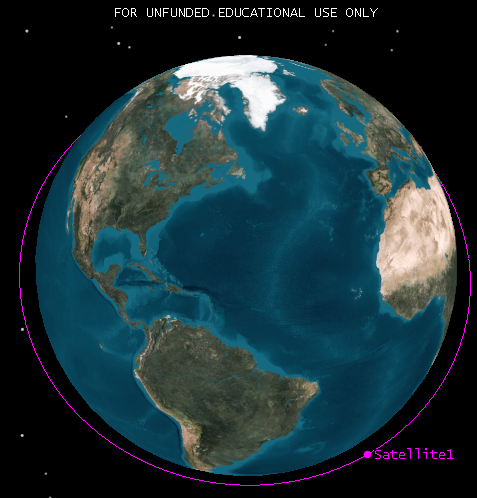
\includegraphics{images/power-bright-orbit}%
\caption{A ``bright'' orbit, where the satellite is exposed to the sun 80\% of the time.  Image generated from STK.}%
\label{fig:power-bright-orbit}%
\end{figure}

\begin{figure}[ht]%
\centering
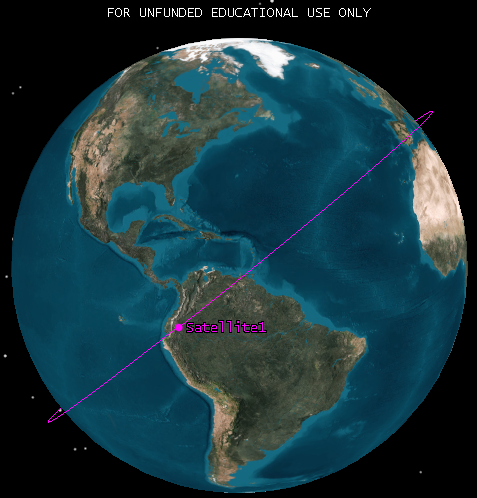
\includegraphics{images/power-dark-orbit}%
\caption{A ``dark'' orbit, where the satellite is exposed to the sun 63\% of the time.  Image generated from STK.}%
\label{fig:power-dark-orbit}%
\end{figure}

The satellite drains the most energy from the battery if it performs a ground station pass (maximum duration: 9.77 minutes) and scientific operation (maximum duration: 5 minutes) during local night:

\begin{equation}
E_{req,batt} = T_{sci} P_{sci} + T_{comm} P_{comm} + (T_e - T_{sci} - T_{comm}) P_{standby} = 3.9 \ \text{Wh}
\label{eq:power-batt-req}
\end{equation}

The excess power is the power actually generated by the panels that does not go into powering the satellite or charging the battery -- in other words, the difference between the power required power and the power actually generated:

\begin{equation}
P_{excess} = P_{panels} - P_{req,panels} = 0.63 \ \text{W (dark)}, 2.57 \ \text{W (bright)}
\label{eq:power-excess}
\end{equation}

It can be useful to model the excess power as an average over the entire orbit, rather than just happening during local day (for first-order approximations of the equilibrium satellite temperature):

\begin{equation}
P_{excess,avg} = P_{excess} \: \frac{T_d}{T_d + T_e} = 0.40 \ \text{W (dark)}, 2.06 \ \text{W (bright)}
\label{eq:power-excess-avg}
\end{equation}

The number of charge-discharge cycles of the battery is approximately equal to the number of orbits that the satellite will have to sustain:

\begin{equation}
N_{cycles} = \frac{T_{year}}{T_{orbit}} = 5500 \approx 6000 \ \text{(with 10\% margin)}
\label{eq:power-num-cycles}
\end{equation}

According to SMAD, the depth of discharge of a lithium-ion battery expected to survive approximately 10,000 cycles should be limited to 60\% \cite[p.~651,~Fig.~21-16]{SMAD}.  This means that the minimum battery size is:

\begin{equation}
E_{batt} \geq \frac{E_{batt,req}}{DOD} = \frac{3.9 \ \text{Wh}}{0.60} = 6.5 \ \text{Wh}
\label{eq:power-batt-size}
\end{equation}

			\subsubsection{Summary of Outputs}
			
			

\begin{table}[ht]
\caption{Outputs to other systems (mass, volume, power consumed, and survival and operating temperatures).\cite[p.~9]{EPS-manual}\cite[p.~11,~21]{PDM-manual}\cite[p.~9]{Battery-manual}\cite[p.~2]{Solar-panel-datasheet}}
\label{tab:power-outputs}
\begin{center}
    \begin{tabular}{|l|l|l|p{0.8in}|p{1in}|p{1.1in}|} \hline
\textbf{Component} & \textbf{Mass (kg)} & \textbf{Volume (U)} & \textbf{Power consumed (W)} & \textbf{Survival temperature ($^\circ$ C)} & \textbf{Operating temperature ($^\circ$ C)} \\ \hline \hline
Solar panels & 0.540 & 0 & 0 & -40 to 80 & -40 to 80 \\\hline
EPS & 0.083 & 0.15 & 0.1 & -50 to 100 & -40 to 85 \\\hline
Battery & 0.256 & 0.2 & 0.1 & -10 to 50 & 0 to 50 \\\hline
PDM & 0.060 & 0.25 & 0.16 & -50 to 100 & -40 to 85 \\\hline \hline
Total & 0.939 & 0.6 & 0.36 & N/A & N/A \\\hline
    \end{tabular}
\end{center}
\end{table}

The power subsystem's outputs were the mass and volume of its components, the power consumed, and the survival and operating temperatures.  The mass and volume were supplied to the Structures subsystem, to ensure that the components would meet the mass and volume constraints of a 3U Cubesat.  The power consumed was taken into consideration in the power budget.  The survival and operating temperatures were used by the Thermal subsystem, to establish the required temperatures in each operating mode.  The values are summarized in Table \ref{tab:power-outputs}.

Some of the components did not contribute to the outputs to other subsystems.  The solar panels are fixed to the sides of the Cubesat, so they do not occupy any of the three units of internal volume, indicated by assigning them a volume of zero.  The battery's low-temperature constraint was not taken into account for the total survival and operating temperature ranges, because the battery has a built-in heater that keeps it above zero degrees Celsius.\cite[p.~12]{Battery-manual}

			\subsubsection{Risks}

The solar panels will supply 4.52 watts on average over an orbit, which is a 28\% margin over the power needs.  However, the EPS is not perfectly efficient.  The connection to the solar panels is the least efficient, with a minimum efficiency of 85\%\cite[p.~9]{EPS-manual}.  When this is taken into account, as few as 3.84 watts may actually be supplied to the battery power bus.  This has a margin of 8.5\% over the satellite's average power needs (which might then be further eroded by inefficiencies in the power lines), which is less than the 18\% margin goal set by Systems, and substantially less than the 30\% margin recommended by JPL.

This system risk is mitigated by the 32\% margin of available power over the standby power need of 2.92 watts.  This provides assurance that the satellite will be power-positive during its standby mode.  Should the satellite find itself unable to meet its power needs with the nominal five minutes of data capture every orbit, it can be commanded to spend more time in standby and downlink modes to restore balance to the power budget.

This strategy brings with it a mission risk: that if the 8.5\% margin is not enough, and the satellite is forced to spend more time in standby mode, it will not spend enough time on data capture and downlink modes to complete its science objectives.

However, as mentioned in Analysis, the available power from the solar panels was calculated for the darkest orbit that the satellite will experience.  For the brightest orbit, the average power generated by the solar panels over the entire orbit increases to 7.42 watts, which, taking the worst-case EPS efficiency into account, results in 6.31 watts reaching the power line.  This has a 78\% margin over the average power required.  In fact, the duration of data capture mode could be increased nearly six-fold to 29 minutes per orbit while maintaining a 30\% margin at 60\% depth of discharge.  This possibility mitigates the mission risk: if the satellite is forced to reduce the duration of data capture and downlink modes during darker orbits to conserve power, it can make up for any shortfalls of captured data during sunnier orbits.

			\subsubsection{Future Work}
The performance of the solar panels and batteries is temperature-dependent.  In particular, the battery becomes more effective as its temperature increases, while the solar panels become less so.  Going forward, it would be useful to perform a more detailed simulation of the satellite that incorporates a thermal model, to more accurately measure the effect of satellite temperature and dissipated excess energy.

\newpage
\FloatBarrier
%%%%%%%%%%%%%%%%%%%%%%%%%%%%%%%%%%%%%%%%%%%%%%%%%%%%%%
% COMM
		\subsection{Communication - ZC}

			\subsubsection{Requirements}
			
\begin{itemize}
\item \textbf{COMM-3.1} The subsystem shall transmit at $19.2\ kb/s$ for uplink and $1.5\ Mb/s$ for downlink. \\
Parent Requirement: COMM-3
\item \textbf{COMM-3.2} The subsystem shall have a bandwidth of $445-455\ MHz$ for uplink and $460-470\ MHz$ for downlink. \\
Parent Requirement: COMM-3
\end{itemize}

The driving requirements for the Communications subsystem are that it should transmit at the data rates and frequencies (Comm-3.2) that are necessary to transmit all data to the ground station. The required frequencies are $445-455\ MHz$ for uplink and $460-470\ MHz$ for downlink. The required data rates are $19.2\ kb/s$ for uplink and $1.5\ Mb/s$ for downlink.

			\subsubsection{Decisions Made}\label{sec:comm_decisions}

The L-3 Cadet Nanosat UHF Radio was chosen for use on DeMi. It transmits at the frequencies and data rates outlined in the requirements. The transceiver has an extra $4\ GB$ of storage that avionics uses in addition to any of its storage. 

Because the transceiver is transmitting and receiving at UHF frequencies, a very common antenna choice is to use a measuring tape antenna that is tuned to the frequency that is desired. Because the antenna works like a quarter-wave monopole, the desired length of the antenna is calculated by dividing the wavelength of the signal by 4. Because the transmitting and receiving frequencies are different, the average of these frequencies is used to compute the wavelength. With a frequency of $465\ MHz$, the wavelength equals $.645$ meters. Then, the length of the antenna can be determined using Equation~\ref{eq:comm-antenna-length}.

\begin{equation}\label{eq:comm-antenna-length}
\lambda = c/f
\end{equation}

In Equation~\ref{eq:comm-antenna-length}, $l$ is the length of the antenna, and $\lambda$ is the wavelength.
Using a wavelength of .645 meters, the desired length of the antenna is about .164 meters. The
gain of this antenna will be approximately 3 dB and the beam width approximately $65^\circ$. DeMi is
using two of these antennas so that communication can occur even if it is rotated 180 degrees
from where it is supposed to be.

The ground station that DeMi communicates with will be the NASA Wallops UHF Ground Station. This ground station is being used because the transceiver chosen for DeMi was also used in the Dynamic Ionosphere CubeSat Experiment, and the ground station that was used in that mission was the NASA Wallops UHF Ground Station. The diameter of the dish is $18.29$ meters, the gain is $35\ dB$ and the beam with is $2.9^\circ$.


\subsubsection{Trade Studies} \label{sec:communications-trade-studies}

The main factor in choosing the transceiver on DeMi is the maximum data downlink rate. Because Payload is generating so much data, the Communications system needs to have a high downlink rate to ensure that all of that data can be sent to the ground. Several options were investigated, and the transceiver with the highest data rate is being used. The transceivers that were considered and their maximum data rates are shown in Table~\ref{table:comm_transceivers}.

\begin{table}[ht]
\caption{Communications Trade Study for Maximum Downlink Data Rate}
\begin{center}
    \begin{tabular}{| c | c |} \hline
    	\textbf{Tranceiver} & \textbf{Maximum Downlink Rate} \\ \hline \hline
Espace Payload Telemetry System & $1\ Mb/s$ \\
AstroDev Li-1 UHF Transceiver & $38.4\ kb/s$ \\
ISIS TXS Small Satellite  S-Band Transmitter & $100\ kb/s$ \\
Tyvak UHF Transceiver & $200\ kb/s$ \\
L-3 Cadet Nanosat UHF Radio & $1.5\ Mb/s$ \\
Microhard MHX2420 Modem & $230.4\ kb/s$ \\ \hline 
    \end{tabular}\label{table:comm_transceivers}
\end{center}
\end{table}

			\subsubsection{Analysis}

The maximum amount of data downlink per pass-by can be calculated by multiplying the downlink data rate and the access duration per pass-by. Given the downlink data rate of $1.5\ Mb/s$, and the access duration of $586$ seconds per pass-by, the maximum amount of data that can be downlinked in one pass-by is $109.9\ MB$. Because the satellite is not always directly above the ground station, the satellite is not always downlinking at the maximum data rate. To account for this, and for space for telemetry data and error correcting code, a margin of a factor of 2 is added, so the maximum amount of data from payload that can be downlinked per pass-by is about $54.95\ MB$. Although this is not as much data as payload is creating, on-board processing is used so that the amount of data that needs to be downlinked is below the maximum amount that is allotted for payload.

A link budget was created in order to determine the link margin for a worst case and a best case for uplink and downlink. The uplink budget and the downlink budget are detailed in Appendix~\ref{app:link_budgets}.

The first calculation for the link budget is to determine the worst case propagation path length. The best case length is $500\ km$ because that is the altitude at which the satellite is orbiting. Figure~\ref{fig:comm_propagation_path} shows how a wave propagates through that atmosphere.

\begin{figure}[ht]
\centering
  \includegraphics[width=5.5in]{images/comm-angles.png}
\caption{Diagram of propagation path of a signal from a satellite \cite[p.~12]{ITU-R}.}
\label{fig:comm_propagation_path}
\end{figure}

In order to determine the propagation path length, $r$, the path length of the first layer and the second layer must be determined and added together. The equation for calculating the path length of a layer is as follows in Equation~\ref{eq:comm_path_length} \cite[p.~9]{ITU-R}.

\begin{equation}\label{eq:comm_path_length}
a_n = -r_n\cos(\beta_n) + \frac{1}{2}\sqrt{4r_n^2\cos^2(\beta_n)+8r_n\delta_n+4\delta_n^2} 
\end{equation}

In this equation, $a_n$ is the path length through layer $n$, $r_n$ is the radius from the center of the Earth to the beginning of layer $n$, $\beta_n$ is the exiting incidence angle, and $\delta_n$ is the thickness of layer $n$.
The angle $\beta_n$ can be calculated using Equation~\ref{eq:comm-exit-angle} \cite[p.~10]{ITU-R}.

\begin{equation}\label{eq:comm-exit-angle}
\beta_{n+1} = \arcsin\biggl(\frac{n_n}{n_{n+1}}\sin(\alpha_n)\biggr) 
\end{equation}

In this equation, $n_n$ is the refractive index of layer $n$, and $\alpha_n$ is the entry incidence angle. Angle $\alpha_n$ can be calculated with the last equation needed in order to calculate the propagation length, Equation~\ref{eq:comm-entry-angle} \cite[p.~9]{ITU-R}.

\begin{equation}\label{eq:comm-entry-angle}
\alpha_n = \pi - \arccos \biggl(\frac{-a_n^2 - 2r_n\delta_n - \delta_n^2}{2a_n r_n + 2a_n \delta_n}\biggr) 
\end{equation}

Values that still need to be defined are $\beta_1$ (because it cannot be calculated using the Equation~\ref{eq:comm-entry-angle}), $\delta_1$, $\delta_2$, $n_1$, and $n_2$. $\beta_1$ is just equal to the complimentary angle to the minimum angle at which the Wallops Ground Station can track, which is $5^\circ$. $\delta_1$ will be equal to the altitude at which the atmosphere ends which one can say is about $100\ km$. $\delta_2$ is just the orbiting altitude minus $\delta_1$. $n_1$, which is simple the refractive index of air, is $1.000293$. The last remaining value to be defined is $n_2$, which is the refractive index of a vacuum, which is just 1. Using these equations, one can find that $a_1$ equals $707\ km$, and $a_2$ equals $1375\ km$. This means that the worst case propagation path length is equal to $2082\ km$. The refraction of the wave in air did not change the path length by very much. Without accounting for the refraction, the path length can be calculated using the equation for $a_n$. In this calculation, $r_n$ equals $r_1$, $\beta_n$ equals $\beta_1$, and $\delta_n$ equals $500\ km$ which is the altitude at which DeMi orbits. These values give a path length equal to $2077\ km$, which is only $5\ km$ shorter than the path length when taking refraction into consideration.

The next value calculated in the link budgets is the Equivalent, Isotropic Radiated Power (EIRP). In order to calculate the EIRP, Equation~\ref{eq:comm-eirp} should be used \cite[p.~476]{SMAD}.

\begin{equation}\label{eq:comm-eirp}
EIRP = P_{tx} + G_{tx} - L_{output} 
\end{equation}

In Equation~\ref{eq:comm-eirp}, $P_{tx}$ is the transmitter power, $G_{tx}$ is the transmit antenna gain, and $L_{output}$ is the output loss which is equal to all losses associated with the transmitter. All of these values can be found in the two link budgets in Appendix~\ref{app:link_budgets}.

Another calculated value in the link budget is the space loss. This is the loss of the signal as it is transmitted through space. It can be calculated using Equation~\ref{eq:comm-space-loss} \cite[p.~476]{SMAD}.

\begin{equation}\label{eq:comm-space-loss}
L_s = 92.45 + 20\log_{10}(r) + 20\log_{10}(f) 
\end{equation}

In Equation~\ref{eq:comm-space-loss}, $L_s$ is space loss, $r$ is the propagation path length, and $f$ is the frequency of the transmitted signal. All of these values can also be found in the two link budget tables in Appendix~\ref{app:link_budgets}.

Equation~\ref{eq:comm-antenna-temp} can be used to calculate the transmitting antenna temperature \cite{pozar}.

\begin{equation}\label{eq:comm-antenna-temp}
T_{antenna} = \eta T_{sky} + (1 + \eta) \frac{T_{sky} + T_{ground}}{2} 
\end{equation}

In Equation~\ref{eq:comm-antenna-temp}, $\eta$ is the antenna efficiency, $T_{sky}$ is the temperature of the space behind the receiving antenna. The temperatures used for uplink are determined by using the background temperature of space. For downlink, the temperature of the Earth is used. $T_{ground}$ is the temperature of the ground around the antenna. For uplink, this is the temperature of the Earth, and for Downlink, it is the background temperature of space.

The system noise temperature, $T_{sys}$, is calculated by adding the transmitting antenna temperature and the receiver temperature \cite{pozar}. The receiver temperature for both cases is unique to the receiver and can be determined by the manufacturer.

The next calculated value is the Receiver Gain to Noise Temperature. This is computed using Eqn.~\ref{eq:comm-gain-to-noise} \cite[p.~477]{SMAD}.

\begin{equation}\label{eq:comm-gain-to-noise}
\frac{G}{T} =  G_{rx} - T_{sys} 
\end{equation}

In Equation~\ref{eq:comm-gain-to-noise}, $G/T$ is the receiver gain to noise temperature, $G_{rx}$ is the receiving antenna gain, and $T_{sys}$ is the system noise temperature. Using $G/T$, the total losses in the system, and EIRP one can determine the receiver carrier to noise ratio \cite[p.~477]{SMAD}.

\begin{equation}\label{eq:comm-carrier-to-noise}
\frac{C}{N_0} = EIRP + \frac{G}{T} - L_{total} + 228.6 
\end{equation}

Using the value from Equation~\ref{eq:comm-carrier-to-noise} and the data rate in decibels, one can calculate the energy per bit to noise ratio \cite[p.~478]{SMAD}.

\begin{equation}\label{eq:comm-energy-to-noise}
\frac{E_b}{N_0} = \frac{C}{N_0} - R_b 
\end{equation}

Finally, the link margin can be determined by subtracting the required energy per bit to noise ratio from the predicted one \cite[p.~478]{SMAD}. The best and worst case link margins for uplink and downlink are shown in Figure~\ref{fig:comm_cases}.


\begin{figure}
\hfill
\subfigure[Best Case Communication]{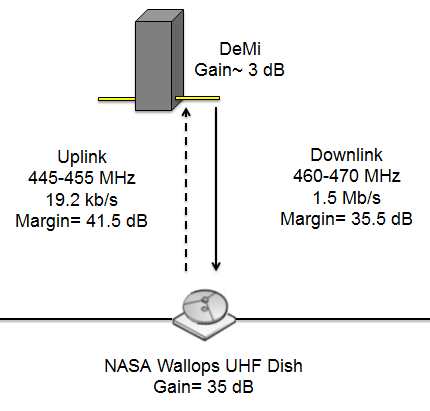
\includegraphics[width=3in]{images/communications-best-case.PNG}}
\hfill
\subfigure[Worst Case Communication]{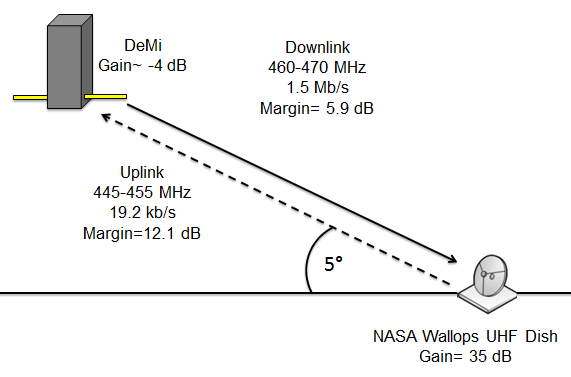
\includegraphics[width=3in]{images/communications-worst-case.PNG}}
\hfill
\caption{Representation of Satellite and Ground Station during a.) Best Case Communication and b.) Worst Case Communication}
\label{fig:comm_cases}
\end{figure}
		
\subsubsection{Summary of Outputs}

There were several outputs during the design process from the Communications subsystem. These outputs include the ground station to the orbits subsystem, which is NASA Wallops UHF Ground Station, the beam width of Wallops UHF Ground Station and DeMi to ADCS, which are $2.9^\circ$ and $65^\circ$ respectively. The operational and survival temperatures of the transceiver to the Thermal subsystem, the power for each mode to the Power subsystem, and the mass and volume to the Structures subsystem are detailed in Table~\ref{table:comm_summary_outputs}.
	
\begin{table}[ht]
\caption{Communications Budgets}
\begin{center}
    \begin{tabular}{|c||c|} \hline
    	\textbf{Output} & \textbf{Value} \\ \hline \hline
    Power (Standby) & 0.51 W  \\
    Power (Data Capture) & 0.51 W \\
    Power (Downlink) & 11.44 W \\
    Power (Uplink) & 0.51 W \\
    Power (Safe Mode) & 0.51 W \\
    Mass & $\sim$ 0.235 kg  \\
    Volume & 0.069 U \\ 
Operating Temperature Range & $-20^\circ$ to $70^\circ$ \\
Survival Temperature Range & $-40^\circ$ to $80^\circ$ \\ \hline 
    \end{tabular}\label{table:comm_summary_outputs}
\end{center}
\end{table}

			\subsubsection{Risks}
			Initially, there were concerns that Communications may not be able to downlink enough of the
data from the Payload; however, Avionics has decided that because of this risk, DeMi will be
doing on-board processing so that less data is required to be downlinked. There is the risk
that there may be a lot of interference at the frequencies that DeMi uses. In order to determine
this, there would have to be a ground station site survey and if there were a problem with
interference, specialized receiver software would have to be developed to mitigate the issue.

			\subsubsection{Future Work}
The main issue to be addressed is testing of measuring tape antennas. There is currently not very much information out there that is available to DeMi concerning them, so research to determine the exact gain, beam width and radiation patterns should be conducted.

\newpage
\FloatBarrier
%%%%%%%%%%%%%%%%%%%%%%%%%%%%%%%%%%%%%%%%%%%%%%%%%%%%%%
% AVIONICS

\subsection{Avionics}

\subsubsection{Requirements - VE}
\begin{itemize}
\item \textbf{AVI-1} Avionics shall provide the necessary interfaces to support all subsystems.\\
Parent Requirements: MLR-3, SYS-2
\item \textbf{AVI-3} Avionics shall write and store data to a mass storage device onboard the satellite.\\
Parent Requirements: MLR-4, SYS-2
\end{itemize}
The main Avionics subsystem requirements are to provide the necessary interfaces, calculations and data storing capability to support functioning of all other subsystems during the mission operation. Other than that Avionics shall be able to recover from potential single event effects and permit software updates and reprogramming in orbit.
However, the most important requirements to consider are the memory and processor capabilities because they are the most difficult to satisfy with a current level of technology.

			\subsubsection{Trade Studies - VE}
There are two main Avionics configurations to be considered that are both able to satisfy subsystem’s requirements. They are presented in Table~\ref{table:avionics_hardware_options}. The major difference between configurations is a capability of the first system to do real time image processing, which results in higher complexity and power consumption of that system (see The Steepest Ascent Mission Interface Computer in Table~\ref{table:avionics_hardware_options}). The second configuration only allows downloading raw images to the ground stations without processing them.


\begin{table}[ht]
\caption{Hardware Options}
\label{table:avionics_hardware_options}
\begin{center}
    \begin{tabular}{| c || p{6cm} | p{6cm} |} \hline
     &	\textbf{Processing on-board} & \textbf{Raw images to the ground} \\ \hline \hline
    Component name & The Steepest Ascent Mission Interface Computer CS-MIC-G-EM & Single Board Computer Motherboard + Pluggable Processor Module with Texas Instruments MSP430F2618 \\ \hline
    Power consumption & 0.5 - 1.25 W & 10 mW \\ \hline
    Capabilities & Telemetry/Telecommand + Real time image processing on FPGA & Telemetry/Telecommand\\ \hline
    Storage Capacity & Up to 16 GB & Up to 2 GB \\ \hline
    Processors & TI MSP430  + Xilinx FPGA (model can be selected) & TI MSP430F2618 \\ \hline
    Interfaces & I2C, SPI, UART & I2C, SPI, UART \\ \hline
    Mass & 62 g & 88 - 114 g \\ \hline 
    \end{tabular}
\end{center}
\end{table}

To select an appropriate hardware, payload requirements should be considered first, since they introduce the most limitations to the processor and memory capabilities.

\begin{table}[ht]
\caption{Camera imaging modes}
\label{table:avionics_modes}
\begin{center}
    \begin{tabular}{| c || p{3cm} | p{3cm} | p{3cm} |} \hline
    	\textbf{Mode} & \textbf{640x480 px ``subframe''} &  \textbf{640x480 px ``subframe''} & \textbf{1280x1024 px  ``full frame''} \\ \hline \hline
    Frame Rate & 100 fps & 10 fps & 10 fps \\ \hline
    Data Rate & 310 Mbit/s & 31 Mbit/s & 131 Mbit/s \\ \hline
    Duration & 30 s & 300 s & 60 s \\ \hline
    Memory Required & 1.14 GB & 1.14 GB & 0.96 GB \\ \hline 
    \end{tabular}
\end{center}
\end{table}

If an approach where all the generated by payload data is sent to ground station without processing it, the payload will be generating around 1 GB of data every time (Table~\ref{table:avionics_modes}). For a given downlink speed of 1.5 Mbit/sec, 600 s is required to downlink all the captured data or 10 ground accesses. Since there is only one ground access every three orbits, in general, this particular approach is considered to be ineffective in terms of payload’s active time.

That is why the second approach is considered. It assumes all necessary calculations to be done onboard and only results are sent to the ground. It dramatically reduces the amount of transferred data to around 10-100 KB instead of gigabytes and enables to implement a closed loop deformable mirror control system.

The next step is Avionics subsystem - its processor. Now we have higher but still reasonable requirements for processing power according to the computation tasks that it will be solving:
1) centroid, delta x and delta y computations, 2) slope reconstruction, and 3) linear algebra for mirror controller.

The Steepest Ascent Mission Interface Computer CS-MIC-G-EM is a good fit for such tasks because it has an FPGA to be configured for image processing and a microcontroller for general tasks such as telemetry and ADCS computations (see Section~\ref{adcs_analysis}).



\subsubsection{Decisions Made - VE}

The CS-MIC-G-EM meets these demands, supporting telemetry and telecommand operations, as well as providing a platform to perform advanced on-board pre-processing of data, allowing for more sophisticated analysis to be performed and more efficient use of available downlink bandwidths. 

Other key features of the CS-MIC-G-EM include its mass storage capability, allowing data from multiple Payload units to be stored centrally and the ability to reprogram the on-board processing units, allowing in-flight updates of algorithms to be performed as well as novel concepts to be supported.

\begin{figure}[ht]
\centering
  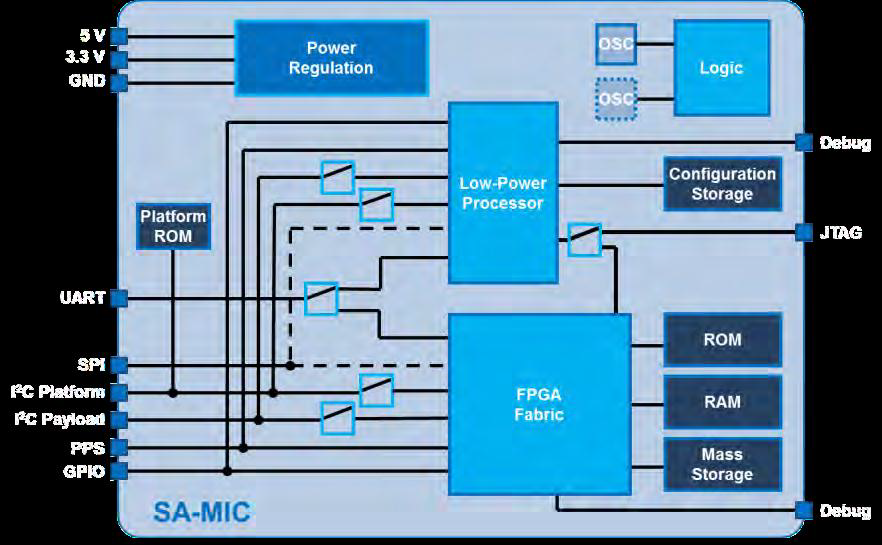
\includegraphics[width=5in]{images/Avionics_fig1.png}
\caption{Structure diagram of Mission Interface Computer CS-MIC-G-EM  \cite{avionics_clyde_space}}
\label{fig:avionics_MIC}
\end{figure}

CS-MIC-G-EM provides a number of options that allow different system architectures to be accommodated. The FPGA Fabric (see Figure~\ref{fig:avionics_MIC}) can be used to implement data processing algorithms, allowing data to be pre-processed before being transmitted to the ground. The attached ROM, RAM and Mass Storage can be used to accommodate more complex algorithms that require buffering of data as well as filter weights/ lookup table values to be stored.

The decision to use CS-MIC-G-EM (see Figure~\ref{fig:avionics_MIC}) is made mainly because it enables the fastest possible onboard image processing \cite{avionics_FPGA} which reduces the amount of data which is sent to the ground and provides with a capability to build a closed loop deformable mirror control system.
General system architecture is shown in Figure~\ref{fig:avionics_architecture}. Selected Mission Interface Computer also allows us to separate telemetry from image processing data. The first is processed on CPU (TI MSP430 microcontroller), which runs an operating system and performs general control tasks, while the latter is done on FPGA (see Table~\ref{table:avionics_hardware_options}) and written into Mass Storage device (see Figure~\ref{fig:avionics_MIC}).

\begin{figure}[ht]
\centering
  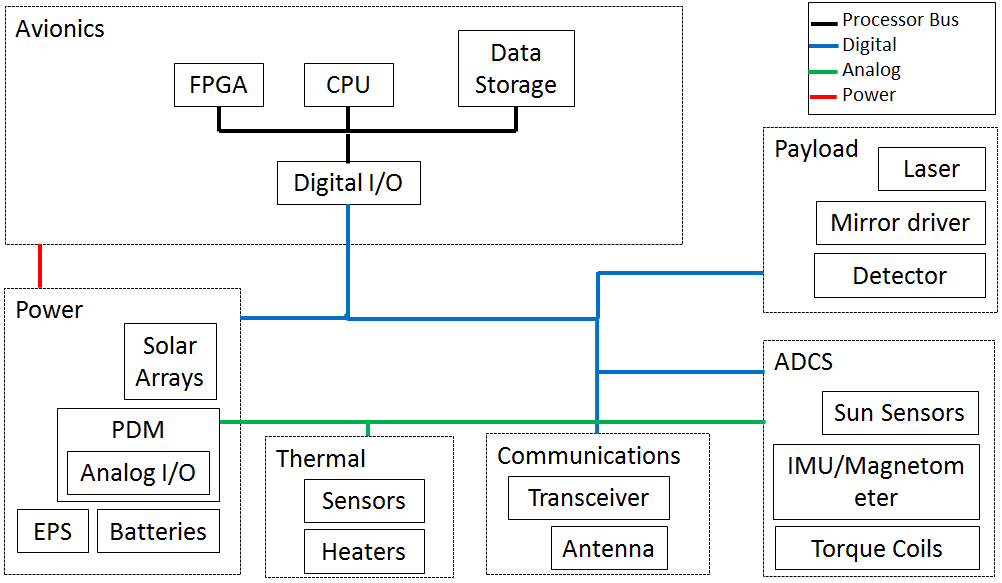
\includegraphics[width=7in]{images/Avionics_fig2.PNG}
\caption{System's structure diagram}
\label{fig:avionics_architecture}
\end{figure}

Another important component to be mentioned is an operating system that is required to control the satellite. Since low power microcontrollers (MSP430) are used, FreeRTOS from Real Time Engineers Ltd. \cite{avionics_RTOS} or Salvo from Pumpkin, Inc. \cite{avionics_pumpkin} real-time operating systems are the best options. Image processing software is supposed to be embedded into FPGA as synthesized hardware architecture which can be done from MATLAB code using HDL Coder.

Avionics provides the following interfaces with other subsystems (see Table~\ref{table:avionics_interfaces}). It is important to mention that all analog interfaces are implemented in a Power Distribution Module (PDM). It allows collecting all the data from analog sensors and sending over a single I2C interface to the Avionics board. PDM implements torque coil drivers as well.


\begin{table}[ht]
\caption{Avionics hardware interfaces with other subsystems}
\label{table:avionics_interfaces}
\begin{center}
    \begin{tabular}{| p{2cm} | l | c | c |} \hline
    	\textbf{Subsytem} & \textbf{Component} & \textbf{Interface} & \textbf{Data rate} \\ \hline \hline
    Payload & Detector (IDS UI-5241LE-M) & GbE & 550 Mbit/s max  \\
     & Mirror driver (BMC Mini-Driver) & USB 2.0 & 480 Mbit/s max \\
     & Laser (ThorLabs CPS 186) & GPIO & -- \\ \hline
    Power & EPS, PDM & 12C & 400 Kbit/s max \\ \hline
    ADCS & 5 sun sensors & Analog (via PDM) & 100 bit/s$^1$ \\
     & ADIS16305 IMU/Magnetometer & SPI & 160 bit/s$^1$ \\
     & Torque coils & Analog (via PDM) & -- \\ \hline
    Thermal & 14 Temperature Sensors & Analog (via PDM) & 100 bit/s$^1$ \\
     & Thermal Heater & Analog (via PDM) & -- \\ \hline
    Comm. & Cadet NanoSat UHF Radio & RS232 & 1.5 Mbit/s \\ \hline 
    \end{tabular}
$^1$Assuming update 10 times per second
\end{center}
\end{table}


			\subsubsection{Summary of Outputs - ZC}

The Avionics subsystem gives values to the Thermal subsystem for operational temperature range, to the Power subsystem for power consumed during the different modes, and to structures for the mass and volume. These outputs are detailed in the chart below (see Table~\ref{table:avionics_summary_outputs}). The survival temperatures of the components are unknown.


\begin{table}[ht]
\caption{Avionics budgets}
\label{table:avionics_summary_outputs}
\begin{center}
    \begin{tabular}{|c||c|} \hline
    	\textbf{Output} & \textbf{Value} \\ \hline \hline
    Power (Standby) & 0.5 W  \\
    Power (Data Capture) & 1.25 W \\
    Power (Downlink/Uplink) & 0.5 W \\
    Power (Safe Mode) & 0.5 W \\
    Mass & 0.062 kg  \\
    Volume & 0.104 U \\ \hline 
    \end{tabular}
\end{center}
\end{table}

			\subsubsection{Risks - ZC}
There are two risks that Avionics currently faces. One risk, that has a high consequence but a very low likelihood, is that the system may not be capable of processing all of the incoming data for payload. Payload is outputting a lot of data, and because the design of the code that will do the process has not yet been done, it is unclear how quickly the Avionics system will be able to process incoming data. The other risk that Avionics currently faces, which is of very low likelihood, but very high consequence, is that it may not be capable of providing the required latency for payload or for ADCS. Research needs to be conducted to determine how fast Avionics can receive and issue orders to ensure that the computer is fast enough for the system. If it is not fast enough there could be major failures in the system because the attitude of the craft is not correct.

			\subsubsection{Future Work - ZC}
The future work that needs to be conducted is that there should be work done to determine a solution to interfacing with payload. The mirror driver interfaces with USB 2.0, however the Avionics board is not able to interface with this. A custom board may be needed to interface the mirror driver with the Avionics board. Research should also be done to ensure that the system can run all of the necessary calculations at the required speed so that all of the payload data can be processed and sent to the ground. If all of the data cannot be processed, it would be difficult to complete the science goals.


\newpage
\FloatBarrier
%%%%%%%%%%%%%%%%%%%%%%%%%%%%%%%%%%%%%%%%%%%%%%%%%%%%%%
% ADCS

\subsection{Attitude Determination and Control System (ADCS) - TN} 
		%%%%%%%%%%%%%%%%%%%%%%%%%%%%%%%%%%%%%%%%%%%%%%%%%%%%%%%%%
			\subsubsection{Requirements}
			The driving requirements of the ADCS design is shown below. A complete requirement document can be found in Appendix A. 
					\begin{itemize}
					\item \textbf{ADCS-1.1} ADCS shall meet 4.7 arcmin/s slew rate requirement of payload imaging technology during external source science operation mode.\\
					Parent Requirement: MLR-3
					
					\item \textbf{ADCS-2.1} ADCS shall provide attitude knowledge of the satellite to an accuracy within 10$^\circ$[TBR]  for communication operations.\\
					Parent Requirement: SYS-4
					\item \textbf{ADCS-2.2} ADCS shall provide attitude control of the satellite to an accuracy within 15$^\circ$ [TBR] for communication operations.\\
					Parent Requirement: SYS-4
					\item \textbf{ADCS-3} ADCS shall provide momentum capability to despin upon launch vehicle separation within 30 days.\\
					Parent Requirement: MLR-4
					\end{itemize}
				The two main requirements during operation modes for the ADCS subsystems are the pointing requirement (15$^\circ$) for communication purpose and the stability (slew rate) requirement (4.7 arcmin/s or 0.08$^\circ$/s) for the payload operation while imaging an external source. This requirement exists to ensure that a photon from the external source stays on the same pixel of the detector during data capture. In addition, the satellite is required to detumble and establish ground station access within a reasonable time frame. This duration is required to be less than 30 days, creating a secondary requirement on the total detumbling time. 
		%%%%%%%%%%%%%%%%%%%%%%%%%%%%%%%%%%%%%%%%%%%%%%%%%%%5
					\subsubsection{Decision Made}
				\paragraph{Control Method}
				Active magnetic control was chosen for this mission due to the low mass and low power requirement and sufficient attitude control performance for both communication requirement and payload science operation. According to documentation on the attitude control system of the 1U CubeSat COMPASS-1 from the University of Applied Sciences, Aachen, Germany, 3 magnetic coils of magnetic moment of  0.097 Am$^2$ can achieve a pointing accuracy of 8$^\circ$ \cite{adcs_compass}. The torque coils can be sized to generate enough torque for a 3U CubeSat. The details of this calculation will be presented in the torque coil specifications and analysis sections below. The stability of this control method is estimated to be $< 0.12^\circ$/s, according to the Illinois Observing Nanosatellite (ION) 2U CubeSat from the University of Illinois \cite{adcs_ion}. The implementation of the active magnetic control the ION mission only includes magnetometer as sensor with low magnetic moment in each torque coils. The performance of the active magnetic control method is expected to improve significantly with the use of more accurate sensors, such as an inertial measurement unit (IMU) and sun sensors, and torque coils with higher magnetic moment. More analysis and testing is needed to determine the stability of the system. 

				\paragraph{Orientation}
				The satellite will be in nadir pointing orientation with the nadir face being one of the two 10 cm $\times$ 10 cm faces. This orientation can be easily achieved by active magnetic control through sending control commands based on sensors readings to the active actuators. The 3U structure of the satellite provides gravity-gradient stability along the long axis in the nadir pointing configuration. By placing an antenna on the nadir face, this orientation facilitates access to the ground station. The satellite will travel with a corner-first configuration, to optimize the amount of power acquired from solar panels (see power section for more details). The orientation of the satellite is illustrated in Figure~\ref{fig:ADCS_orientation} below. 
			
			\begin{figure}[!h]
				\centering
				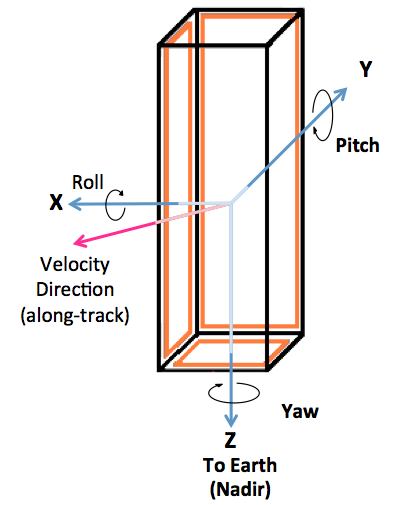
\includegraphics[scale=0.5]{images/ADCS_coord.png}
				\caption{Satellite orientation with respect to nadir direction and velocity vector}
				\label{fig:ADCS_orientation}
			\end{figure}
				
				\paragraph{ADCS sensors and actuators}
				A summary of the sensors and actuators used in the ADCS is presented in Table~\ref{tab:ADCS_sensors} below. 
			% Table generated by Excel2LaTeX from sheet 'Sheet1'
\begin{table}[htbp]
  \centering
  \caption{ADCS Sensors and Actuators}
    \begin{tabular}{|r|r|r|r|r|}
    \hline
    \textbf{Sensors/Actuators} & \textbf{Quantity} & \textbf{Vendor} & \textbf{Performance}  &\bigstrut\\
    \hline
    Sun sensors & 5     & CubeSat shop & \multicolumn{1}{r}{- Field of view: 114$^\circ$} &  \bigstrut[t]\\
          &       &       & \multicolumn{1}{r}{- Accuracy: $< 0.5^\circ$} &  \bigstrut[b]\\
    \hline
    Magnetometer & 1     & Analog Devices  & \multicolumn{1}{r}{- Dynamic range: ± 3.5 gauss} &  \bigstrut[t]\\
          &       & (ADIS16405) & \multicolumn{1}{r}{- Initial bias: ± 4 mgauss} &  \bigstrut[b]\\
    \hline
    IMU   & 1     & Analog Devices  & \multicolumn{1}{r}{- Dynamic range: ±300$^\circ$/s} &  \bigstrut[t]\\
          &       & (ADIS16405) & \multicolumn{1}{r}{- Initial bias: 3$^\circ$/s} &  \\
          &       &       & \multicolumn{1}{r}{- In-run bias stability: 0.007$^\circ$/s} &  \bigstrut[b]\\
    \hline
    Torque coils & 3     & N/A   & \multicolumn{1}{r}{- Max magnetic moment: 0.060, 0.063 $Am^2$} &  \bigstrut\\
    \hline
    \end{tabular}%
  \label{tab:ADCS_sensors}%
\end{table}%

			For attitude knowledge, a combination of sensors was chosen: sun sensors, magnetometers, and IMU.  The sun sensors are low mass and low power attitude sensors that provides accurate sun angle during day time, providing the orientation of the satellite relative to an inertial frame. Five sun sensors will be places on the faces of the satellite other than the nadir face. These sensors provides an accuracy of $< 0.5^\circ$ and a wide field of view of 114$^\circ$. The magnetometer will be used to measure the local geomagnetic field to compute the magnetic moment needed to generate needed restoring torques. In addition, the magnetometer will be used as the main attitude sensing device during eclipse periods. An IMU is used to measure the angular rate of the satellite to provide more accurate vibration knowledge to yield a robust vibration damping control loop. The IMU and magnetometer are in the same sensor unit from Analog devices. Both sensors have initial biases that can be corrected for through computation. 

For actuation, 3 custom-made orthogonal torque coils will be used for 3-axis stabilization control. The coils will be sized to meet the mass and power constraint of the satellite and to provide sufficient magnetic moment to counter environmental disturbances. More detailed calculation will be presented in the analysis section. The specifications of the torque coils are presented in Table~\ref{tab:ADCS_torquecoils} below.
			% Table generated by Excel2LaTeX from sheet 'Sheet2'
\begin{table}[htbp]
  \centering
  \caption{Torque coils specifications}
    \begin{tabular}{|r|r|r|}
    \hline
    Direction & Z     & X, Y \bigstrut\\
    \hline
    Size  & 10 cm $\times$ 10 cm  & 10 cm $\times$ 30 cm \bigstrut\\
    \hline
    Quantity & 1     & 2 \bigstrut\\
    \hline
    Turns & 500   & 300 \bigstrut\\
    \hline
    Current & 0.12 A & 0.07A \bigstrut\\
    \hline
    Wire Gauge & 28 AWG & 28 AWG \bigstrut\\
    \hline
    Magnetic moment & 0.60 Am$^2$ & 0.63 Am$^2$ \bigstrut\\
    \hline
    \end{tabular}%
  \label{tab:ADCS_torquecoils}%
\end{table}%
				\paragraph{System Schematics and Interfaces}
				The system schematics are shown in Figure~\ref{fig:ADCS_schem}. The IMU/magnetometer unit, which will be mounted on an interface board, and the sun sensors will be read out through the analog channels of the power distribution module. The module will be used as an interface to the avionics subsystem. The attitude knowledge data will be processed in the avionics subsystem. Combining with the local magnetic field, the magnetic moment vector needed for the torque coils can be computed. This information will be sent to the torque coils through the Power Distribution Module (PDM), into the torque coil driver. The driver consists of a current driver and an H-bridge, which controls the current in each coils and their directions, respectively. 
			
			\begin{figure}[!ht]
				\centering
				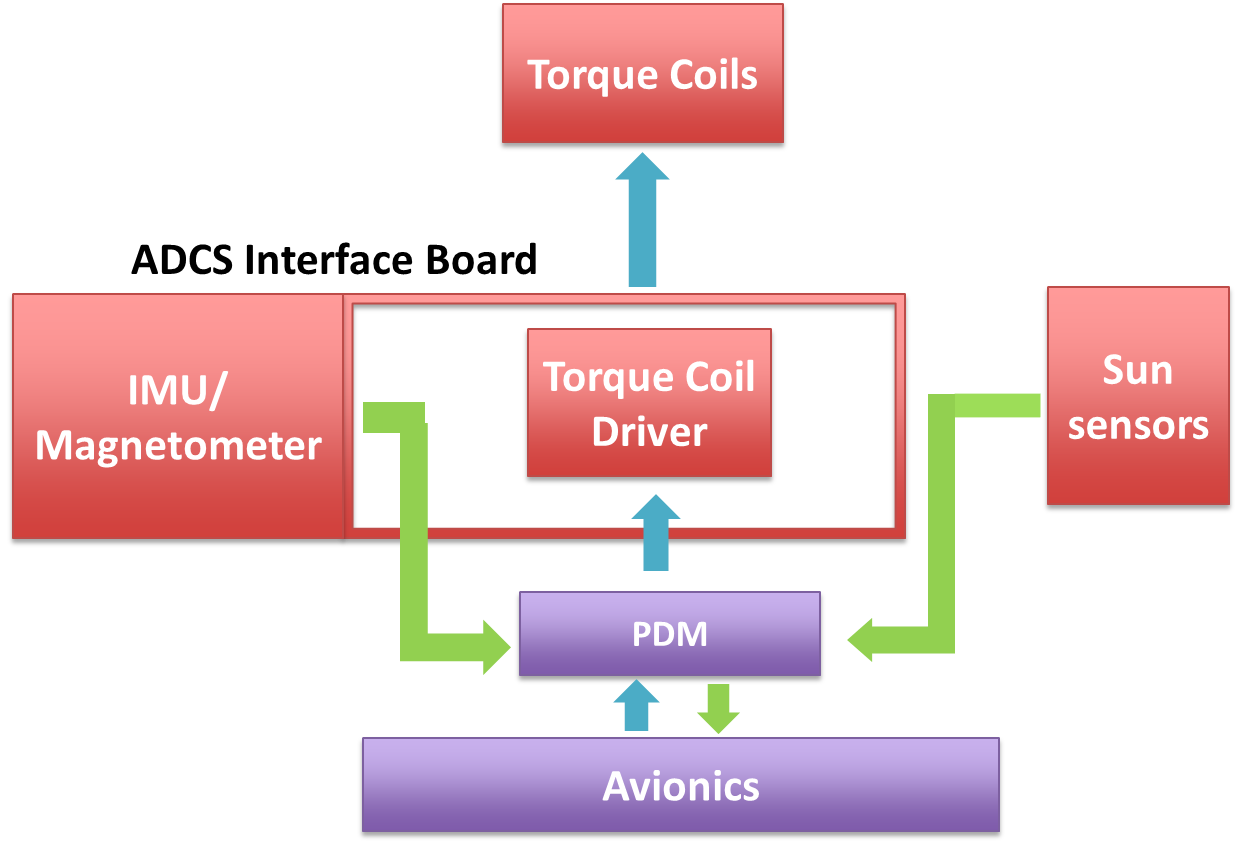
\includegraphics[scale=0.5]{images/ADCS_schem.png}
				\caption{ADCS components interactions and Avionics interface}
				\label{fig:ADCS_schem}
			\end{figure}
		%%%%%%%%%%%%%%%%%%%%%%%%%%%%%%%%%%%%%%%%%%%%%%
			\subsubsection{Trade Studies}
			Several control methods were considered in the design process of the ADCS system: passive magnetic control, passive magnetic control, and control using reaction wheels. The main trades to be considered are mass, power usage, pointing accuracy, and pointing stability capability. 

In passive magnetic control, restoring torque is generated through the alignment of the satellite magnetic moment with the local geomagnetic field. The magnetic moment is created through the use of permanent magnets. Hysteresis rods are used for vibration damping. This control option requires low mass and no power. Based on past CubeSat missions, the pointing accuracy of a passive magnetic control system in the same scale as DeMi can achieve 10$^\circ$ –- $20 ^\circ$, sufficient for communication requirement purpose \cite{adcs_survey} \cite{adcs_smad1}. However, there are limitations in the ability to stabilize the satellite. Passive magnetic control systems stability performance is not reliable because the hysteresis rods do not provide fast and robust vibration damping. The expected stability achieved by this method is $1^\circ$ –- $10 ^\circ$/s \cite{adcs_survey}. Since the satellite will only have access to the external sources for a short amount of time, this method is not practical for capturing light from the stars. In addition, this control method limits the possible orientation of the satellite to only the direction along the local magnetic field. In a LEO orbit of 40$^\circ$ inclination such as that of DeMi’s, the direction of the local magnetic field varies at different orbital parameters. This variation causes difficulties in placing antenna and external source aperture so that ground station access and external source capture can be guaranteed. 

Reaction wheels provide robust 3-axis stabilization control of the satellite. This control mechanism provides high accuracy ($~ 0.0001^\circ$ -– $1^\circ$) in pointing direction and quick response in vibration damping providing high stability (0.05$^\circ$/s) \cite{adcs_smad1}. However, the necessary sensors and actuators require high mass and power usage. The main mass contribution and power draw are from the reaction wheels. In addition, magnet torquers are also needed to desaturate reaction wheels, adding more mass and power strain on the system. This option is not practical for a small satellite such as DeMi. 

A summary of the control methods performances is presented in table~\ref{tab:ADCS_trade} below. Based on this information, active magnetic control was chosen for this mission. 

\begin{table}[htbp]
  \centering
  \caption{Performance of control methods considered in trade studies}
    \begin{tabular}{|p{4cm}|p{3cm}|p{3cm}|p{3cm}|}
    \hline
          & \textbf{Passive Magnetic Control} & \textbf{Active Magnetic Control} & \textbf{Reaction Wheels Control } \bigstrut\\
    \hline
    \textbf{Mass } & Low   & Moderately Low & High  \bigstrut\\
    \hline
    \textbf{Power} & Low   & Moderately Low & High \bigstrut\\
    \hline
    \textbf{Pointing  Accuracy} &  10$^\circ$ -- 20$^\circ$ &  1$^\circ$ -- 10$^\circ$ &  0.0001$^\circ$ -- 1$^\circ$ \bigstrut\\
    \hline
    \textbf{Pointing Stabilization} & 1$^\circ$/s  -- 10$^\circ$/s & $<$ 0.12 $^\circ$/s & $<$ 0.05 $^\circ$/s \bigstrut\\
    \hline
    \end{tabular}%
  \label{tab:ADCS_trade}%
\end{table}%




			
			\subsubsection{Analysis}
			\label{adcs_analysis}
				\paragraph{Environmental Torque Calculation}
				The main environmental disturbances on orbit are gravity gradient, magnetic field, aerodynamics drag, and solar radiation pressure. The governing equations of these external sources are presented in details in SMAD ADCS section \cite{adcs_smad2}. Using the satellite properties and orbital parameters, the upper bound of these values can be computed and presented in Table~\ref{tab:ADCS_envtorque}. The exact environmental torques varies with the satellite position and orientation. A preliminary simulation was constructed to compute these values and will be discussed briefly int the ADCS Future Work section.This simulation has not been refined or modified.
				
				% Table generated by Excel2LaTeX from sheet 'Sheet3'
\begin{table}[htbp!]
  \centering
  \caption{Maximum Environmental Torque Estimation}
    \begin{tabular}{|r|r|}
    \hline
    Gravity Gradient & 1.60E-08 Nm \bigstrut\\
    \hline
    Magnetic Field & 1.80E-05 Nm \bigstrut\\
    \hline
    Atmospheric Drag & 2.70E-07 Nm \bigstrut\\
    \hline
    Solar Pressure & 5.50E-09 Nm \bigstrut\\
    \hline
    Total Torque & 1.80E-05 Nm \bigstrut\\
    \hline
    \end{tabular}%
  \label{tab:ADCS_envtorque}%
\end{table}%

			\paragraph{Torque coil sizing calculation}
			Magnetic control relies on the torque provided by the aligning of the satellite magnetic moment and the local magnetic field. Equation~\ref{eqn:ADCS_torque} shows the governing equation of magnetic control, where $\vec{T}$ represents the generated torque vector, $\vec{\mu}$ is the satellite magnetic moment, $\vec{B}$ is the local geomagnetic field vector. 
			
			\begin{equation}
				\vec{T} = \vec{\mu} \times \vec{B}
				\label{eqn:ADCS_torque}
			\end{equation}
			
			Taking the torque vector to be the total environmental torque, Equation~\ref{eqn:ADCS_torque} yields the required maximum magnetic moment of the coils to be $~ 0.6$ A$\cdot$m$^2$. The magnetic moment of each coil can be calculated from the coil parameters as shown in Equation~\ref{eqn:ADCS_mu} below, where $\mu$ is the magnitude of the magnetic moment generated by the coil, $I$ is the current in the coil, $N$ is the number of turns, and $A$ is the area of enclosed by the coil. 
			
			\begin{equation}
				\mu = I \cdot N \cdot A
				\label{eqn:ADCS_mu}
			\end{equation}
			
			Since the area of each coil is chosen to be the same as the size of each of the face of the satellite, the main trade of the design is the number of turns and current in each coil. This corresponds to a mass/power trade. The results of the torque coil sizing are presented above in Table~\ref{tab:ADCS_torquecoils} in Decision Made section. 
			
			\paragraph{Detumbling Analysis}
				Using the Princeton Satellite Systems MATLAB simulation, the momentum unloading as a response to an initial angular rate can be computed. The input parameters are the magnitude and direction of initial angular momentum, the direction of magnetic moment, and the gain of the control loop. The initial momentum was calculated by assuming an initial angular rate. The magnetic moment direction is the direction of the torque coils. The control gain is adjusted so that the maximum magnetic moments along all 3 axes are less than the maximum magnetic moments provided by the torque coils. The detumbling time can be calculated through determining the time where the momentum in all direction is less than an arbitrary low threshold. 

The simulation was run with an initial angular rate of 10$^\circ$/s, magnetic moment along x, y, z and a control gain of $k =0.008$. The angular momenta and magnetic moments are presented in Figure~\ref{fig:ADCS_detumbling}.
			
			\begin{figure}[!ht]
				\centering
				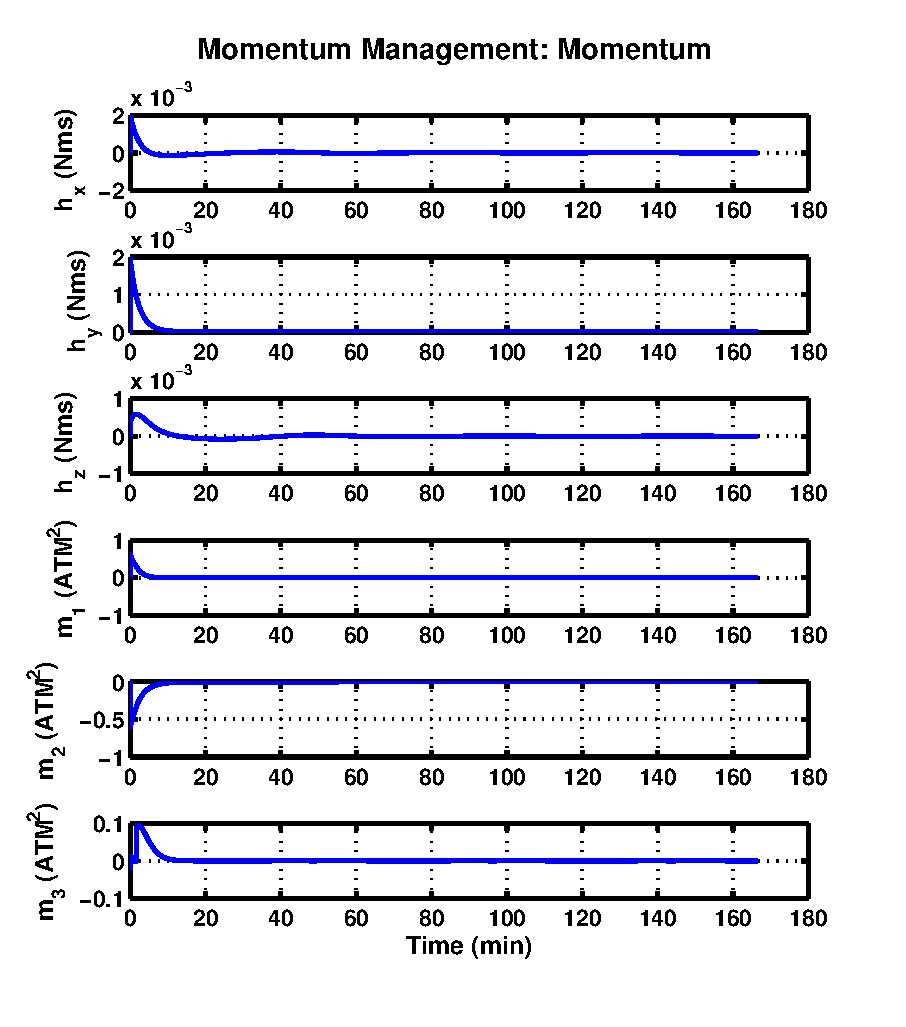
\includegraphics[scale=0.8]{images/ADCS_detumbling.eps}
				\caption{Momentum and magnetic moment during detumbling period}
				\label{fig:ADCS_detumbling}
			\end{figure}

			The maximum magnetic moment needed in x, y, z are 0.6092 Am$^2$ , 0.6052 Am$^2$, 0.0938 Am$^2$, respectively, which is within the range of magnetic moment the torque coils can provide. The total detumbling time is less than 1 orbit (94 minutes). 
			
			\paragraph{Ground Access Duration}
			The duration of access to ground station was computed using an STK model. The orbit was set to a LEO orbit of 500 km altitude and an inclination of 40$^\circ$. The satellite configuration is set to be in nadir pointing with a possible offset of 8$^\circ$. The design of the antenna is a monopole antenna of 16 cm long (beamwidth of 65$^\circ$), transmitting at 465 MHz and receiving at 450 MHz. The corresponding length/wavelength ratio is 0.24. The ground station is set to NASA Wallops flight facility UHF parabolic dish of 18.29 m diameter (beamwidth of 2.9$^\circ$). A screen shot of the STK model is presented in Figure~\ref{fig:ADCS_STK}. 
			
			\begin{figure}[!ht]
				\centering
				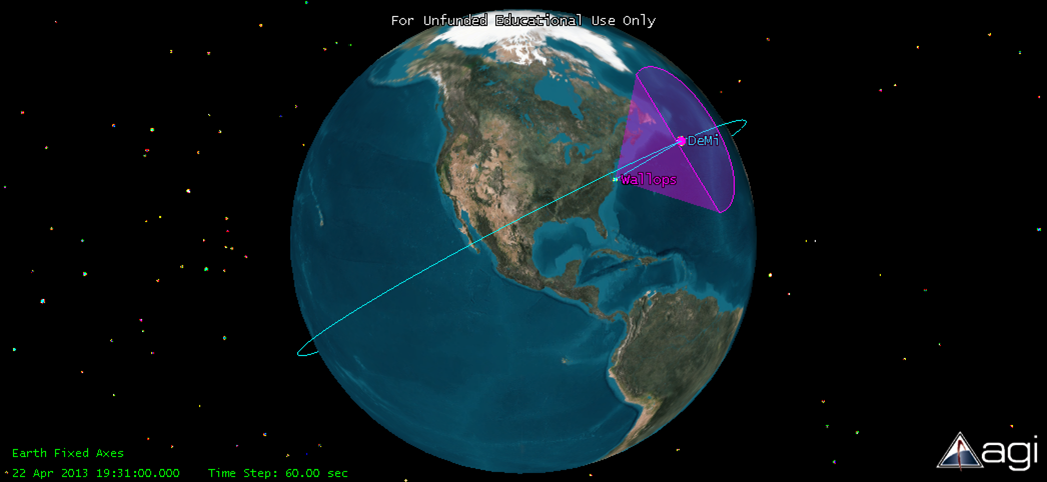
\includegraphics[scale=0.8]{images/ADCS_STK.png}
				\caption{Ground access STK model}
				\label{fig:ADCS_STK}
			\end{figure}
			
			The simulation was run over the course of a day. There are a total of 5 access opportunities of about 9 minutes each. The total ground station access time per day is about 45 minutes. The exact access duration varies with each orbit. 
		
			\subsubsection{Summary of Budgets}
			
			The mass, power, and volume budgets of the ADCS system are presented in Table~\ref{tab:ADCS_budget}. As expected, the main power draw and mass contribution of the ADCS system is from the torque coils. The power presented in the table (1.35 W) represents the power required by the actuators in the worst case scenario. The interface board takes up the most volume (0.318 U) and will stacked in the chassis along with the avionics boards. 
			
		% Table generated by Excel2LaTeX from sheet 'Sheet4'
\begin{table}[htbp]
  \centering
  \caption{ADCS budgets}
    \begin{tabular}{|r|r|r|r|}
    \hline
    \textbf{Component} & \textbf{Volume} & \textbf{Mass} & \textbf{Power} \bigstrut\\
    \hline
    IMU/Magnetometer & 4.49 $cm^3$ & 0.016 kg & 0.21 W \bigstrut\\
    \hline
    Sun sensors & 6.530 $cm^3$ & 0.02 kg & 0.25 W \bigstrut\\
    \hline
    Torque coils & 58.32 $cm^3$ & 0.52 kg & 1.35 W (max power)\bigstrut\\
    \hline
    Interface board & 248.0 $cm^3$ & 0.17 kg & -- \bigstrut\\
    \hline
    \multicolumn{1}{r}{} & \multicolumn{1}{r}{} & \multicolumn{1}{r}{} & \multicolumn{1}{r}{} \bigstrut\\
    \hline
    Total ADCS system (with margin) & 318 $cm^3$ (0.318 U) & 0.73 kg & 1.81 W \bigstrut\\
    \hline
    \end{tabular}%
  \label{tab:ADCS_budget}%
\end{table}%


			\subsubsection{Risks}
			%The main design risk in the ADCS system is the pointing stability requirement and the mass and power budget. As previously mentioned, the stability of the satellite will need to be $<$ 0.08$^\circ$/s for payload science operation of capturing light from a star. The sensors and actuators are expected to provide this performance based on the survey of past CubeSat missions. However, more analysis through simulation and testing will need to be implemented to determine the exact performance of the system. The second risk is due to the narrow margin on the power budget of the whole system. To compensate for this, the mass of the torque coils is higher than previously expected. More iterations are needed to determine the optimal power consumption and mass of the torque coils. 
			One risk in the design of the ADCS system is the ability to achieve the stability requirement of 0.08$^\circ$/s for payload science operation of capturing light from an external source. As previously mentioned, a similar CubeSat active magnetic control system (from ION from University of Illinois) can achieve the stability of $<$0.12$^\circ$/s. The design of DeMi ADCS system is more robust than that of ION and is expected to yield sufficient stability control of the satellite (see Decision Made section for more details). However, this stands as a design risk and can be mitigated through further analysis and testing. This is a low likelihood risk since the ADCS design can be modified with little effect on the whole system. The consequence of this risk is also moderately low since external source light capturing is not the primary objective of the mission. 
			\subsubsection{Future Work}
			The main future work of the ADCS system is to simulate the flight condition through computation of the external disturbance torques at each position on orbit on the satellite frame of reference. The next step is to create a control loop that takes these environmental torques as inputs to compute the needed magnetic moment of each of the 3 torque coils. 
			
			A preliminary MATLAB/Simulink simulation was constructed with the first objective to the simulate flight condition and a second objective of creating an attitude control loop, which will be implemented after the first objective is achieved. A high level block diagram of the simulation is presented in Figure~\ref{fig:ADCS_simulink}. The simulation takes the orbital parameters and satellite properties as inputs to compute the external torques based on the equations presented in SMAD ADCS section \cite{adcs_smad2}. The magnetic field model used is the International Geomagnetic Reference Field (IGRF) 11. The gravitational field and air density are currently assumed to be constant at the chosen altitude. 
			
						
			\begin{figure}[!ht]
				\centering
				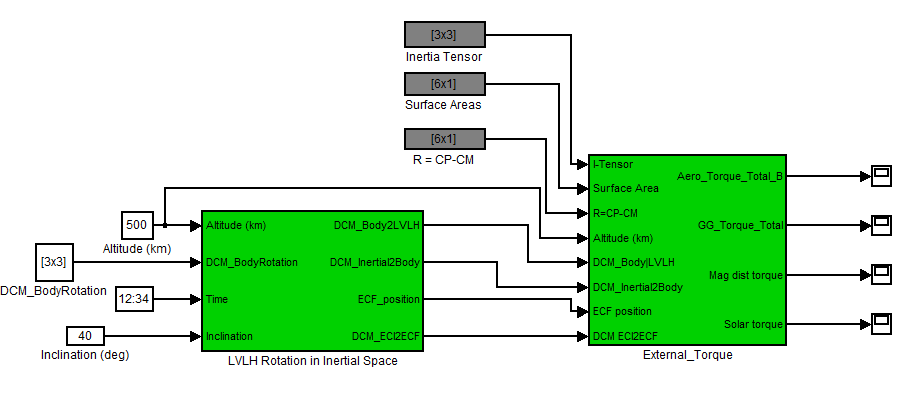
\includegraphics[width=\textwidth]{images/ADCS_simulink.png}
				\caption{High level block diagram of on-orbit external torques simulation}
				\label{fig:ADCS_simulink}
			\end{figure}
			
			There are still several modifications that needs to be made to refine the simulation as it is still in an early stage. For example, the satellite orientation is currently chosen arbitrarily instead of from the result of a close loop control. No eclipse calculation has been taken into account in the torque calculations. The simulation will be further developed and verified as part of the future work on the ADCS system. 
		
		
\newpage
\FloatBarrier
%%%%%%%%%%%%%%%%%%%%%%%%%%%%%%%%%%%%%%%%%%%%%%%%%%%%%%
% THERMAL

\subsection{Thermal - IM}
		
\subsubsection{Requirements}

\begin{itemize}
	\item \textbf{THM-1} The thermal subsystem shall ensure that all components are kept within their survival temperature ranges for the duration of the mission.
	\\
	Parent Requirements: SYS-2, MLR-3
\item \textbf{THM-2} The thermal subsystem shall ensure that all operating components are kept within their operating temperature ranges.
\\
Parent Requirements: SYS-2, MLR-3
\item \textbf{THM-3} The thermal system shall be able to monitor the temperatures of all key components.
\\
Parent Requirement: SYS-2
\end{itemize}


\subsubsection{Analysis/Results}

The analysis of the thermal environment of the satellite took into consideration the radiation fluxes from the sun and earth (albedo and infrared) on all six faces of the CubeSat as shown in Figure~\ref{fig:thermal-environment}. For each face, an energy balance was carried out and the average energy over all faces used to determine the average temperature of the satellite. The energy balance equations were as follows:

\begin{equation}
Q_{in} + Q_{internal} = Q_{out} \rightarrow [\alpha(S + S_A) + \epsilon S_{IR}] A + Q_{internal} = A_S \epsilon \sigma T^4
\label{eq:thermal-balance}
\end{equation}

Where $\alpha$, $\epsilon$, and $A_S$ are the absorptivity, emissivity, and area of the surface, $\sigma$ is the Stefan-Boltzmann constant, and $Q$ and $S$ correspond to the energy and radiation fluxes respectively. Values for radiation flux over the course of an orbit were taken from The New SMAD \cite[p.~688,~table~22-11]{SMAD}, the main text for this course. Temperatures were calculated for two extremes of thermal environment, the cold case, $\beta$ = 0; and hot case, $\beta$ =45, where $\beta$ is the angle subtended by the orbit relative to the sun.  Different values of radiation flux correspond to each value of $\beta$.

The operating and survival temperatures of other subsystems are shown in Table~\ref{table:thermal-inputs}. These figures were used to determine the desired temperature range of the satellite during each mode of operation. The results of the analysis are shown in Table~\ref{table:thermal-results}. These show that during the cold case, the satellite will experience temperatures below the operation and survival temperatures of the payload during data-capture and other modes respectively.

\begin{figure}[ht]%
\centering
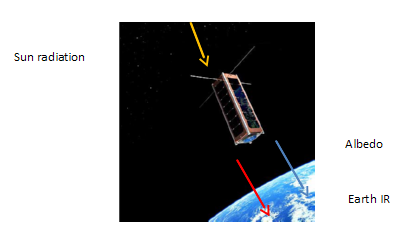
\includegraphics{images/thermal-environment}%
\caption{Thermal environment of satellite considered in analysis.\cite{satnews}}%
\label{fig:thermal-environment}%
\end{figure}

\begin{table}[ht]%
\caption{Operating and survival temperatures of different subsystems and components.}
\label{table:thermal-inputs}
\begin{tabular}{|p{1.5in}|l|l|}\hline
\textbf{Equipment} & \textbf{Operating Temperature} [$^\circ$C] & \textbf{Survival Temperature} [$^\circ$C] \\\hline
\textbf{Payload} & 0 to 35 & -10 to 70 \\\hline
\textbf{ADCS} & -20 to 40 & -20 to 40 \\\hline
\textbf{Avionics} & -25 to 85 & -25 to 85\\\hline
\textbf{Batteries} (have internal heaters) & 0 to 50 & -10 to 50\\\hline
\textbf{Solar Arrays} & -40 to 80  & -50 to 100 \\\hline
\textbf{Communications} & -20 to 70 & -40 to 80 \\\hline
\end{tabular}
\end{table}

\begin{table}[ht]%
\caption{Results of the thermal analysis for hot and cold cases.}
\label{table:thermal-results}
\begin{tabular}{|l|r|r|r|r|r|}\hline
\textbf{Mode} & \textbf{Data Capture} & \textbf{Standby} & \textbf{Uplink} & \textbf{Downlink} & \textbf{Safe} \\\hline
\textbf{Operating temp.} [$^\circ$C] & 0 to 35 & -10 to 40 & -10 to 40 & -10 to 40 & -10 to 40 \\\hline
\textbf{Temp. Cold case} [$^\circ$C] & \textbf{-3.68} & \textbf{-13.40} & \textbf{-13.40} & 5.79 & \textbf{-15.72} \\\hline
\textbf{Temp. Hot case} [$^\circ$C] & 21.99 & 14.72 & 14.72 & 29.31 & 13.02 \\\hline
\end{tabular}
\end{table}

\subsubsection{Trade Studies}

Based on the results of the thermal analysis, the need to augment the thermal control was evident. Amongst the myriad of possible options, the inclusion of a heater, thermal blanket, and surface coating were more feasible for a CubeSat mission given the limited mass, volume, and power available. The payload’s detector was the main component whose temperature needed to be kept above the average satellite temperature for most modes of operation, so either a heater or thermal blanket needed to be chosen as the primary thermal control for the payload.

The heater being considered was a model HK5586 polyimide thermofoil heater from Minco (see Figure~\ref{fig:thermal-heater}). It takes up an area of 4.50 cm x 2.54 cm, operates within -200 to 200 $^\circ$C, and with an input voltage of 3.3V, would require a maximum wattage of 0.83 W. 

\begin{figure}[ht]%
\centering
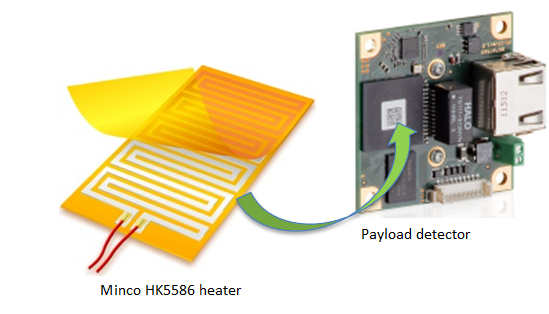
\includegraphics{images/thermal-heater}%
\caption{Thermofoil heater and payload detector.\cite{minco,ids-imaging}}%
\label{fig:thermal-heater}%
\end{figure}

Computing the heat exchange between the heater and the detector, we obtained values for the average power required by the heater to keep the detector above 0 $^\circ$C during data capture mode, and above -10 $^\circ$C during other modes. The equation used:

\begin{equation}
P_{req} = \frac{\text{Energy transferred}}{\text{Time}} = \frac{m_{sat} Cp_{sat} (T_{min} - T_{sat})}{\text{Time}}
\label{eq:thermal-power-required}
\end{equation}

Where a maximum of ten seconds is allowed for the detector to attain desired temperatures, $m$ and $Cp$ are the mass and effective specific heat capacity of the detector, and $T_{min}$ corresponds to the minimum operational and survival temperature during data capture and other modes respectively. The results are shown in Figure~\ref{fig:thermal-power-usage}. Besides downlink mode, the heater will require power ranging from 0.44 to 0.75W which is a significant percentage of the average power available to the entire satellite.

\begin{figure}[ht]%
\centering
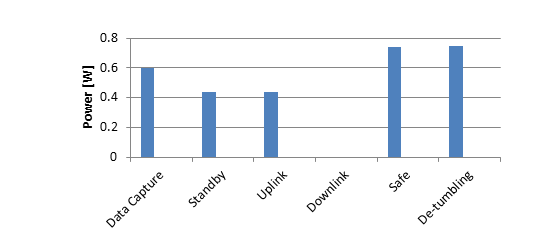
\includegraphics{images/thermal-power-usage}
\caption{Power usage by heater during different modes of operation.}%
\label{fig:thermal-power-usage}%
\end{figure}

For the thermal blanket option, we considered aluminized 25 gauge polyester with nylon scrim from Dunmore. Some of the advantages of this option are that it does not require power, and its mass requirement is significantly low.

In order to determine the amount of insulation needed, a lumped parameter model for the thermal diffusion through the thermal blanket was used. Temperature of the inner face of the MLI is given by

\begin{equation}
T = T_\infty + (T_i- T_\infty)e^{-t/\tau}, \tau = m \times Cp \times R_{ext}
\label{eq:thermal-inner-MLI}
\end{equation}

Where $\tau$ is the time constant for temperature decay, $R_{ext}$ is the thermal resistance to external heat flux, and $T_i$ and $T_\infty$ are the initial temperature of the inner face and average temperature of the satellite respectively. In order to achieve a time constant of approximately the duration of eclipse, two layers of insulation will be required. The results are shown in Figure~\ref{fig:thermal-decay}.

\begin{figure}[ht]%
\centering
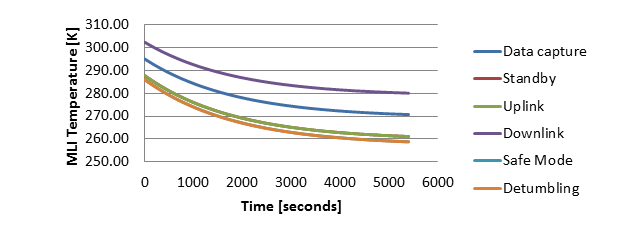
\includegraphics{images/thermal-decay}%
\caption{Temperature decay of inner face of MLI for different modes of operation.}%
\label{fig:thermal-decay}%
\end{figure}

\subsubsection{Design/Budget}

Given the results of the aforementioned analysis, the thermal blanket was chosen for primary thermal control. Initially, the thermal subsystem chose dispense with idea of a payload heater, and use solely the MLI for thermal control, but after further discussion with other subsystems, it was agreed upon to still have the heater installed. The rationale behind this decision was that in the event that the average satellite temperature falls below the predicted value, the heater would be used to augment the action of the thermal blanket.
 
Thus, the design will include a double layer thermal blanket surrounding the payload, aluminized 25 gauge polyester with nylon scrim taking up approximately 1g and 0.8cm$^3$ of mass and volume respectively. In addition, the heater will be attached to the detector within the thermal blanket as shown in Figure~\ref{fig:thermal-heater}.  Furthermore, in order to fully meet the third requirement of the subsystem, the temperatures of key components of other subsystems will be monitored via thermal sensors.  These components are listed in Table~\ref{table:thermal-sensors} below.

\begin{table}[ht]%
\centering
\caption{Key components and their corresponding number of thermal sensors required.}
\label{table:thermal-sensors}
\begin{tabular}{|l|r|}\hline
\textbf{KEY COMPONENTS} & \textbf{Sensors needed} \\\hline
Sun sensors & 5 \\\hline
Torque coils & 3 \\\hline
ADCS interface board & 1 \\\hline
DMs + Driver & 1 \\\hline
Detector & 1 \\\hline
Laser & 1 \\\hline
Electronic Power System & 1 \\\hline
Power Distribution Module & 1 \\\hline
\textbf{Total} & \textbf{14} \\\hline
\end{tabular}
\end{table}

The thermal sensors chosen are model 44004 precision thermistor elements from Omega, each of volume 0.04 cm$^3$ and mass 0.4 g. Fourteen in all, they will each draw power of about 0.5 $\mu$W and operate within a temperature range of -80 to 120 °C. As shown in Figure~\ref{fig:thermal-thermistor} they consists of a bead and a tail; the bead will be attached to the surface of the component whose temperature is being measured, and the tail goes to the avionics board.

\begin{figure}[ht]%
\centering
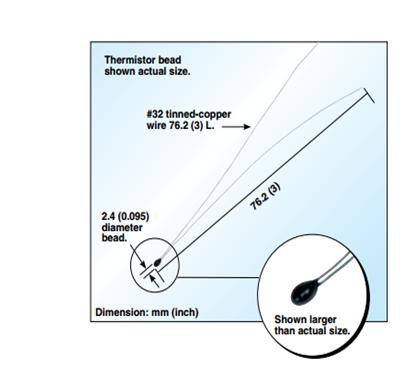
\includegraphics{images/thermal-thermistor}%
\caption{Precision Thermistor elements -- model 44004 (Omega.com).\cite{omega}}%
\label{fig:thermal-thermistor}%
\end{figure}

In addition, the zenith and nadir faces will be painted with Chemglaze Z306 ($\alpha= 0.98, \epsilon = 0.89$) in order to improve their absorptivity-emissivity ratio from 0.9 to 1.1.

In summary, the mass, volume, and power budget will be as shown in Table~\ref{table:thermal-outputs}.  The heater will be used only in emergency to supplement the thermal control action of the multi-layer insulation. As such, the thermal subsystem will take up 8 g, negligible power, and 2 cm$^3$ when the heater is not in use.

\begin{table}[ht]%
\centering
\caption{Mass, volume and power budget for the thermal subsystem.}
\label{table:thermal-outputs}
\begin{tabular}{|l|l|l|l|}\hline
& \textbf{Mass} [g] & \textbf{Power} [mW] & \textbf{Volume} [cm$^3$] \\\hline
\textbf{Thermistors} & 5.4 & 0.007 & 0.6 \\\hline
\textbf{Thermal blanket} & 1.1 & -  & 0.8 \\\hline
\textbf{Heater} (emergency use only) & 1.5 & 770 & 0.6 \\\hline
\textbf{Surface coating} & - & - & - \\\hline
\textbf{Total} & \textbf{8.0} & \textbf{0.007 to 770} & \textbf{2} \\\hline
\end{tabular}
\end{table}

\subsubsection{Future Work}

For further work, an analysis which considers thermal gradient across satellite should be paramount. Based on the CAD model of the satellite created by the Structures subsystem and the known average heat fluxes on the faces of the CubeSat, a steady-state thermal analysis of the satellite was begun during the course of the project. However, due to time constraints, the analysis was not completed before the end of the project.

\newpage
\FloatBarrier
%%%%%%%%%%%%%%%%%%%%%%%%%%%%%%%%%%%%%%%%%%%%%%%%%%%%%%
% STRUCTURES

\subsection{Structures - JL}

\subsubsection{Requirements}

The primary requirements of the Structural subsystem are that the entire satellite fit within the dimensional requirements imposed by the cubesat requirements. The requirements are listed below:

\begin{itemize}
\item \textbf{STR-1} The primary structure shall be a 3U CubeSat. \\
Parent Requirement: SYS-3

\item \textbf{STR-1.1} The structure shall be 340.5mm in length ($x$) by 100.0mm in width ($y$) by 100.0mm in height ($z$).\\
Parent Requirement: STR-1

\item \textbf{STR-1.2} The structure shall not exceed 6.5mm in protrusion normal to the surface of the 100mm cube.\\
Parent Requirement: STR-1

\item \textbf{STR-1.3} The center of gravity of the structure shall be no more than 20mm offset from centerline.\\
Parent Requirement: STR-1

\item \textbf{STR-1.4} The structure shall be composed of Aluminum 7075 or 6061.\\
Parent Requirement: STR-1

\item \textbf{STR-1.5} The structure shall have rails of hard anodized aluminum.\\
Parent Requirement: STR-1

\item \textbf{STR-1.6} The structure shall pass a minimum of 1 fit check.\\
Parent Requirement: STR-1

\item \textbf{STR-2} The structure shall provide space and attachment points for the payload, the avionics system, the power system, and the ADCS.\\
Parent Requirement: SYS-1

\item \textbf{STR-2.1} Attachment points shall ensure no relative motion of attached modules during launch as well as during nominal operating conditions.\\
Parent Requirement: STR-2

\item \textbf{STR-2.2} Interfaces shall survive thermal expansion and contraction across a range of $-150^\circ$ C to $60^\circ$ C.\\
Parent Requirement: STR-2

\item \textbf{STR-2.3} The lowest resonant frequency of all CubeSat components shall be higher than the resonant frequency of the launch vehicle.\\
Parent Requirement: STR-2

\item \textbf{STR-3} The structure shall facilitate interfaces between other subsystems.\\
Parent Requirement: SYS-3

\item \textbf{STR-4} The structure shall not interfere with payload field of view.\\
Parent Requirement: PLD-2

\item \textbf{STR-5} The structure shall allow for workmanship screening of the avionics boards.\\
Parent Requirement: MS-1

\end{itemize}

The driving requirements are STR-1 in order to adhere to cubesat requirements and secure a launch, STR-2 and STR-4 as they are required for the system to fulfill the mission.

\subsubsection{Trade Studies}
The first trade study that was performed was to determine whether or not an off the shelf structural chassis would need to be purchased or if a custom designed chassis would be more suitable to the mission of DeMi. The Pumpkin 3U Skeletonized Chassis was considered as the off the shelf option as it has had numerous successful flights on previous cubesat missions. Additionally, it is designed to easily interface with the numerous off the shelf products that would be used by the various other subsystems.

\begin{figure}[!ht]
\centering
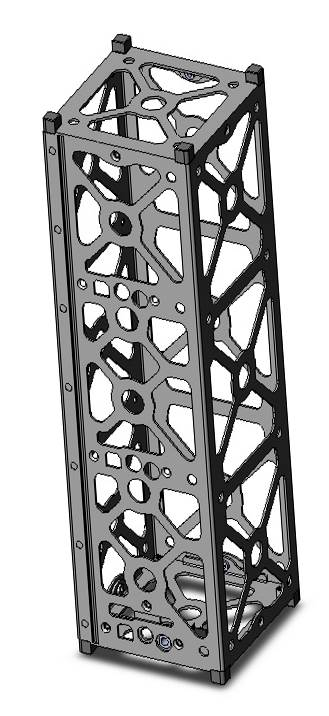
\includegraphics[width=2in]{images/STR-1.jpg}
\caption{Pumpkin 3U Skeletonized Chassis. Image from CubeSatKit\cite{cubesatkit}}
\label{fig:str-1}
\end{figure}

Additionally, due to the necessity for any deployable to be structurally constrained by the satellite, a trade study was conducted to determine whether a commercially available communications antenna would be purchased, or if a custom antenna would be mounted to the satellite. The most readily available antenna products for cubesats are the ISIS deployable Antenna~\cite{cubesatshop}, pictured in Figure~\ref{fig:str-2-3}.

\begin{figure}[!ht]
\hfill
\subfigure {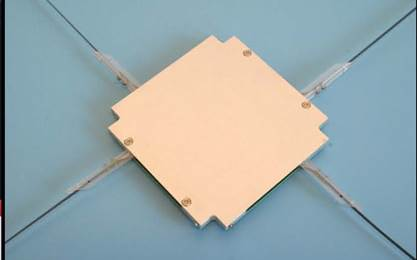
\includegraphics[width=3in]{images/STR-2.jpg}}
\hfill
\subfigure {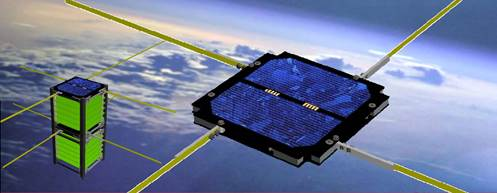
\includegraphics[width=3in]{images/STR-3.jpg}}
\hfill
\caption{Photo and Artist’s rendering of ISIS Deployable Antenna. Images from ISIS~\cite{isis-image}}
\label{fig:str-2-3}
\end{figure}

\subsubsection{Decisions Made}
The chosen chassis for the DeMi mission was the Pumpkin 3U Skeletonized Chassis due to the fact that it has had numerous successful flights in the past and is a readily available package that can interface with the cubesat components that have been chosen by the various other satellite subsystems.

The antennas that will be used for communication will be custom made, simple 0.5 inch wide, 18.25 cm long steel tape measure fastened to the bottom, nadir pointing plate of the satellite. The feed point will be connected such that 16.4 cm of the length will be used as for communication and the remaining tape length used for mounting the antennas. The tape measure will be fastened to the side of the satellite while stowed within the P-POD by a length of nylon wire and will be melted during the de-tumbling phase of the mission by a power resistor. Once the wire has melted, the antennas will be deployed.

\begin{figure}[!ht]
\centering
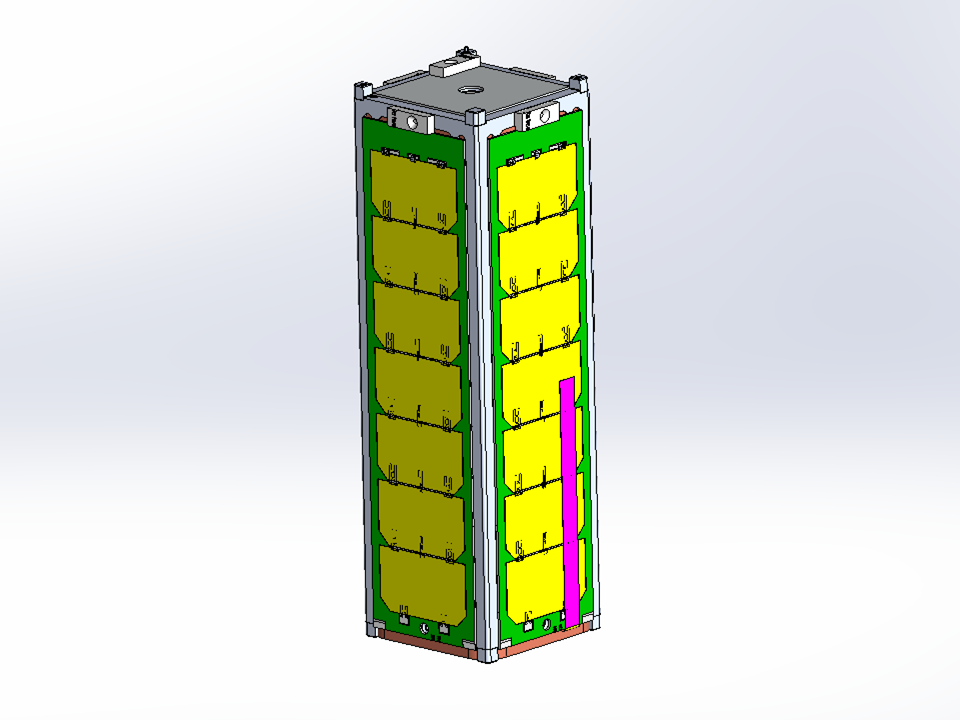
\includegraphics[width=4in]{images/STR-4-Revised.png}
\caption{Antennas in stowed configuration. Antenna highlighted in pink. Image generated by SolidWorks.}
\label{fig:str-4}
\end{figure}

\begin{figure}[!ht]
\centering
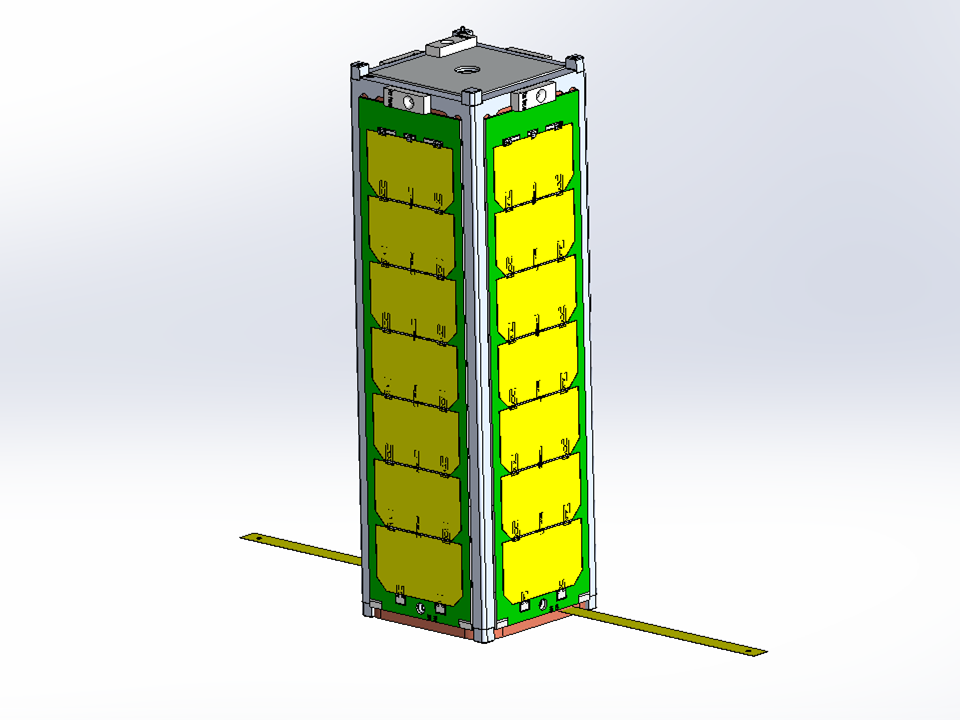
\includegraphics[width=4in]{images/STR-5-Revised.png}
\caption{Antennas in deployed configuration. Image generated by SolidWorks.}
\label{fig:str-5}
\end{figure}

A custom antenna was chosen as opposed to the available commercial option due primarily to the fact that the design and implementation of such an antenna is very simple. This would save on the total cost of the satellite. Additionally, the commercial option is overbuilt for the purposes of the DeMi mission, having additionally complexity that was determined to be unnecessary for the satellite. By using a simpler, custom design, less mass needs to be allotted for the communications subsystem. Finally, there is confidence that this simplified design will work due to the fact that simple tape measure antennas have been flown numerous times before and have been proven to be successful~\cite{uhf-cubesat, cubesat-leo}.

\subsubsection{Analysis}

In order to ensure that the entire system fit within the dimensional constraints outlined by the cubesat requirements, and that the center of mass of the entire system was within an acceptable range, the system stack was modeled in SolidWorks. Models for the various boards were acquired by their respective vendors, or stand-ins were modeled based on dimensions and masses provided by each subsystem. Once the masses were finalized and the component locations finalized, SolidWorks was able to provide an estimated center of mass of the entire system.

\begin{figure}[!ht]
\centering
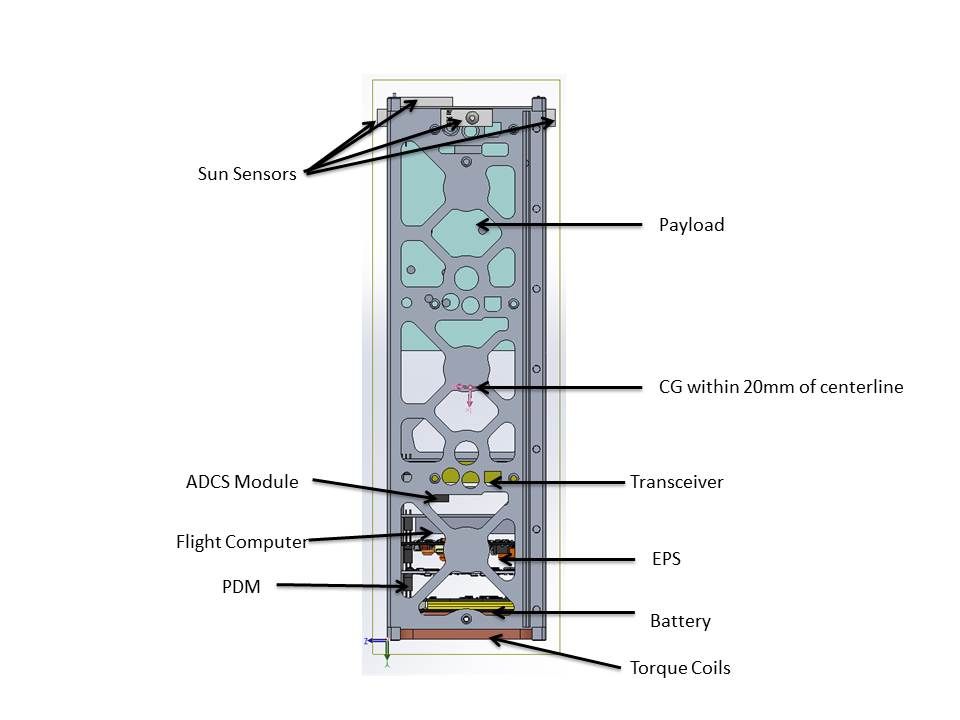
\includegraphics[width=5in]{images/STR-6-revised.jpg}
\caption{System stack with CG depicted. Image Generated from SolidWorks.}
\label{fig:str-6}
\end{figure}


\begin{figure}[!ht]
\centering
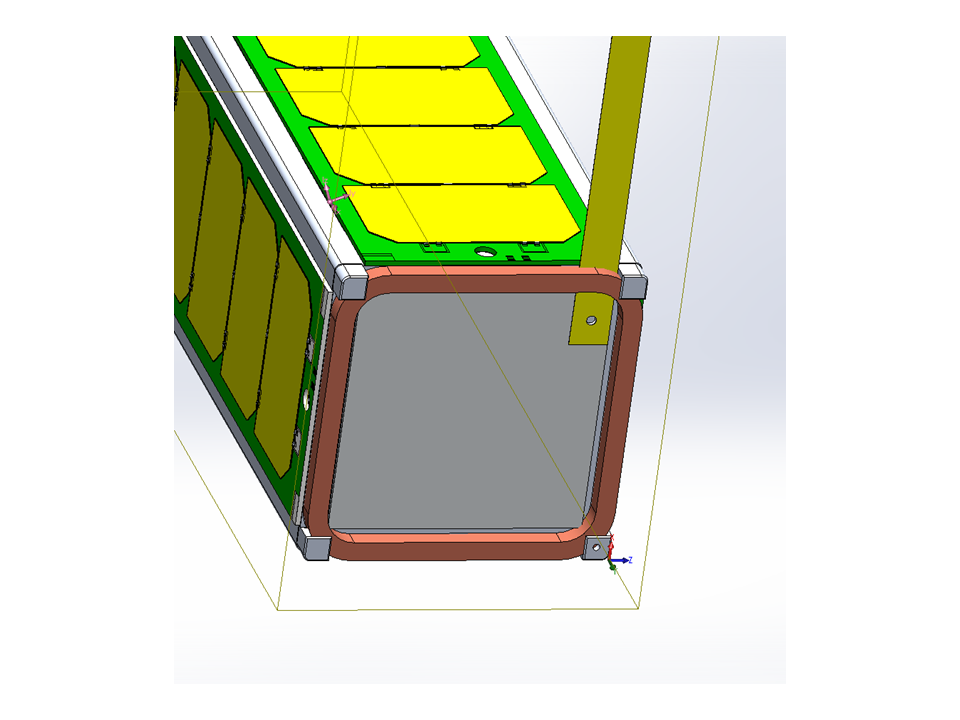
\includegraphics[width=5in]{images/STR-7(2).png}
\caption{Nadir Pointing Face Depicted with Axes Shown. Image Generated from SolidWorks.}
\label{fig:str-7}
\end{figure}


As shown in the image, the center of mass is within the 20 mm range of the geometric center. The exact coordinates are $X$: 48.18mm, $Y$: -154.42 mm, and $Z$: -55.80 mm, with axes as defined in the image below.

The boards of the system stack are fastened together with steel male-female threaded hex standoffs, due to their strength, easy availability, and ease of use--allowing the configuration of the boards to be changed easily. Due to the fact that the CubeSat boards are able to stack in any order thanks to the common bus connection, the placement of the boards within the stack was primarily driven by the location of the center of gravity (CG) requirement discussed earlier. In order to keep the CG centered along the long axis, the $Y$-axis in the model, the system stack was pushed to the far extremity away from the Payload box, as the Payload itself has the greatest subsystem mass. Within the system stack, the battery and transceiver are the heaviest components, weighing an estimated 260 grams and 235 grams respectively. This led to the necessity of separating them within the stack. If they were both at the topmost extreme of the stack, the CG could have been moved too far. If they were both near the center of the satellite assembly, the CG may have been biased toward the payload box.  The rest of the components are arranged by subsystem for simplicity and organization, from top to bottom as depicted in the image below: Power, Avionics, ADCS, Communications.

\begin{figure}[!ht]
\centering
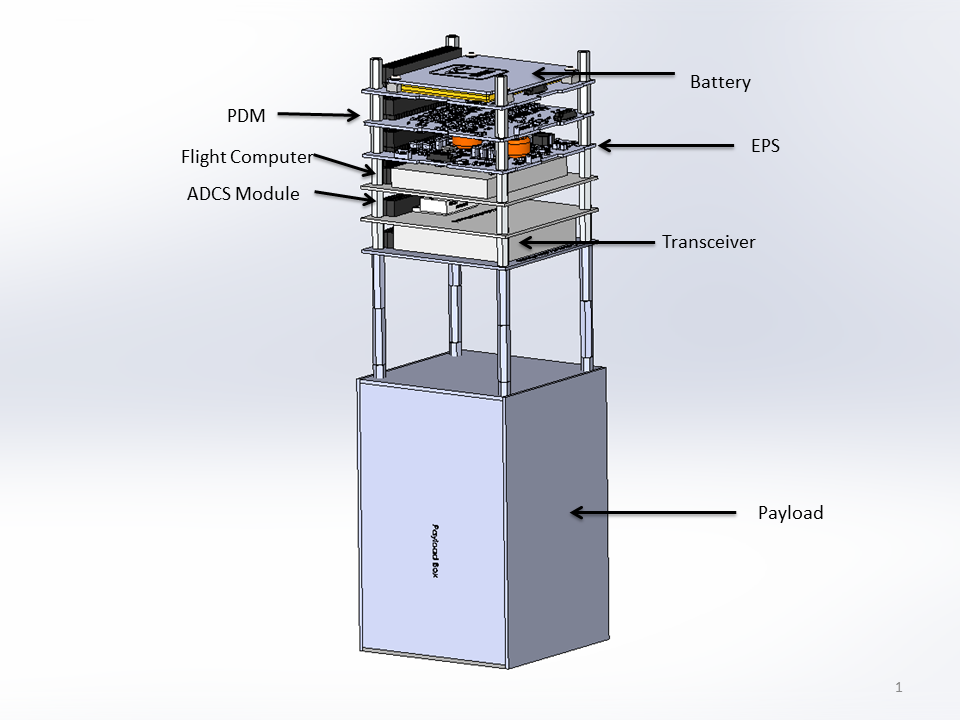
\includegraphics[width=6in]{images/STR-8.png}
\caption{System stack with components highlighted. Image Generated from SolidWorks.}
\label{fig:str-8}
\end{figure}

Component placement within the Payload box was dictated by component locations acquired from the Payload team. All components are placed on aluminum posts that will be custom machined such that the center of all the components is aligned with the long axis, the $Y$-axis, of the satellite. This is primarily to satisfy the CubeSat CG requirement.

\begin{figure}[!ht]
\centering
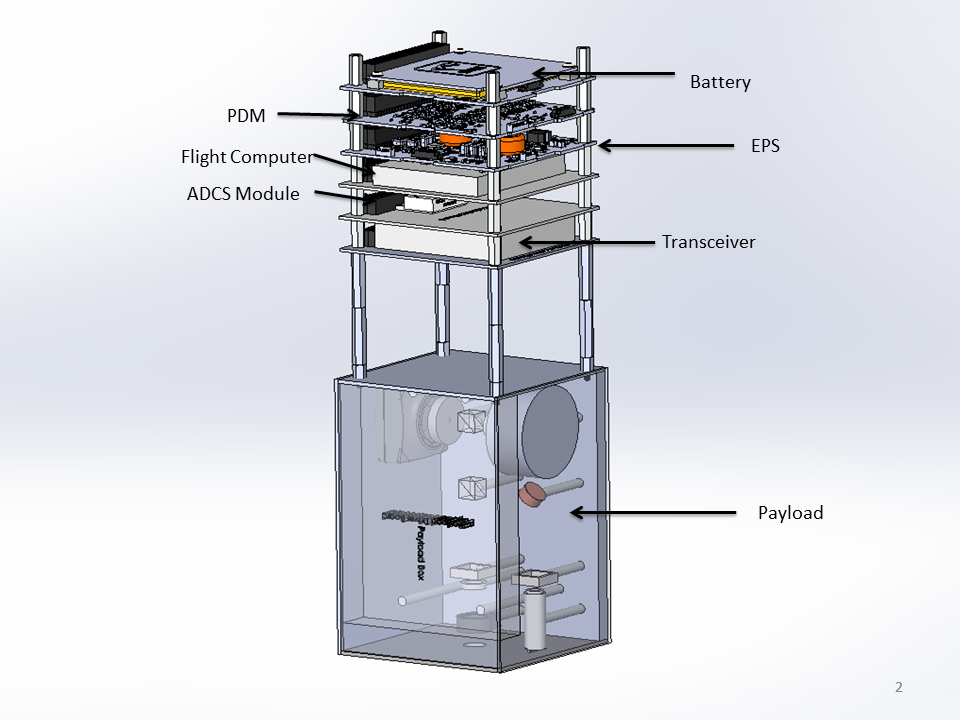
\includegraphics[width=6in]{images/STR-9.png}
\caption{System Stack with Payload box components visible. Image Generated from SolidWorks.Additionally, the Payload driver board is mounted to the top panel of the Payload box, again for CG considerations.}
\label{fig:str-9}
\end{figure}

\begin{figure}[!ht]
\centering
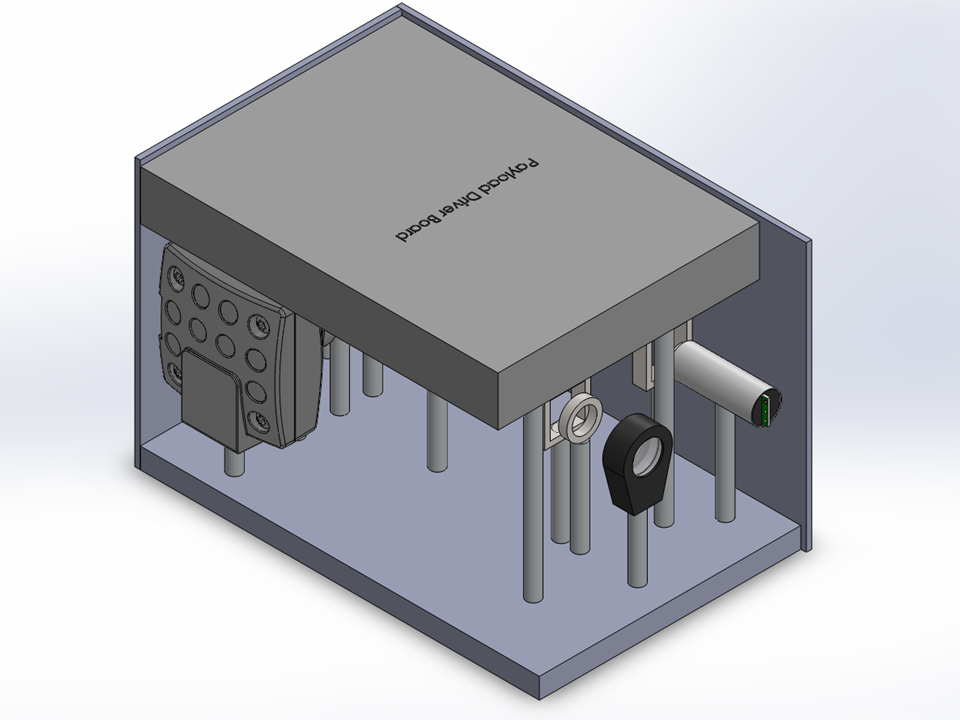
\includegraphics[width=4.5in]{images/STR-10.png}
\caption{Internal view of Payload box. Driver board visible. Image Generated from SolidWorks.}
\label{fig:str-10}
\end{figure}

\begin{figure}[!ht]
\centering
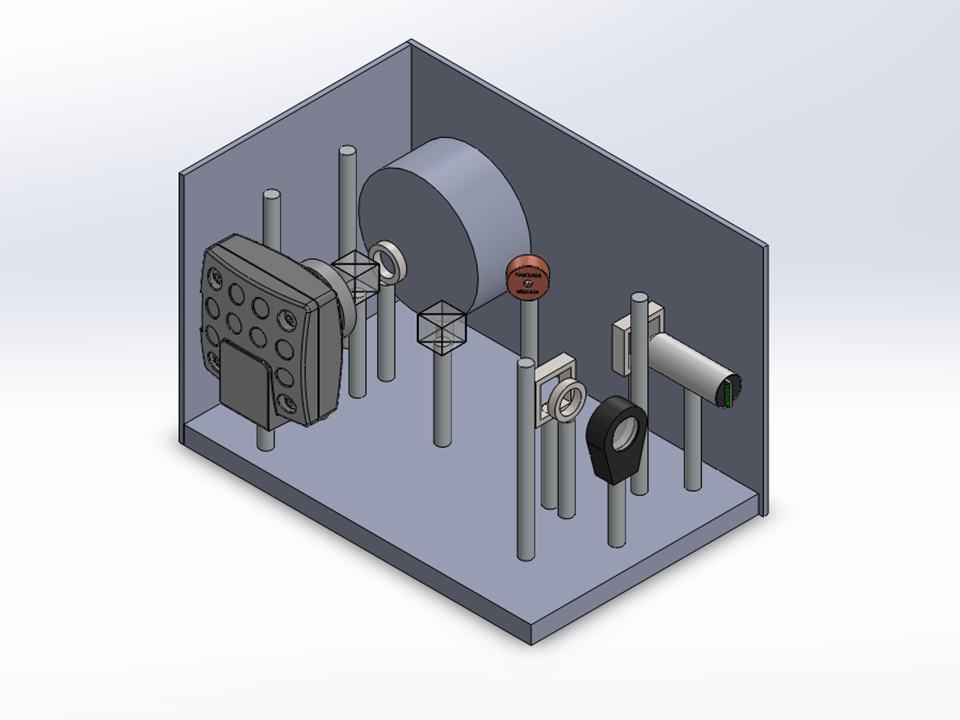
\includegraphics[width=4.5in]{images/STR-11.png}
\caption{Internal view of Payload box. Driver board hidden for view of components. Image Generated from SolidWorks.}
\label{fig:str-11}
\end{figure}

\subsubsection{Summary of Outputs}
The structural subsystem outputted a SolidWorks model for the thermal subsystem to carry out a thermal analysis that took into account component placement.
Images of the payload box and the internal components was given to the payload subsystem for use in illustrating the layout of the subsystem.
Additionally, the inertia tensor was given to the ADCS subsystem for analysis.

\subsubsection{Risks}
At this point in the design stage, the greatest risk is that center of mass moves out of the accepted range as the system design matures. The center of mass provided above is within the acceptable limit, but is sensitive to component placement and mass, two factors that are very likely to change as the design process continues. This risk, while unlikely at the moment, poses a high risk in that if it is out of range, the satellite cannot launch.
Another potential risk is that the satellite will not survive the launch environment (launch loads, vibrations, etc.). This risk is deemed moderately likely with a high risk, as Finite Element Modeling (FEM) and structural analyses still needs to be carried out before the likelihood of the risk can be fully assessed. Considering that most of the components used in the satellite are off the shelf components designed for application to a cubesat mission, the most likely components to fail are the few custom components (the antenna mounts and restraining system, the ADCS board), and the standoffs that support the system stack. The risk is high however in that if something does break and/or connections between key components are severed, the entire mission could potentially be jeopardized.

\subsubsection{Future Work}
Immediate future work to be carried out by the Structural subsystem is a finite element modeling of the system and structural analysis to ensure that the satellite and all the components will survive the launch environment in their current configuration. Additionally, the structural model will need continual updates as the system matures.

%%%%% CONCLUSION

\section{Conclusion - AW}

In this report, it has been shown that a low-cost, quick-access mission can be carried out on a 3U CubeSat platform in order to demonstrate MEMS deformable mirror imaging technology on-orbit.  At the current design stage, the system weighs 3.26 kg.  Applying AIAA Mass Growth Allowance values for Preliminary Design \cite{mission_aiaa}, the mass increases to 3.90 kg.  This is in accordance with the maximum mass of 4 kg for a triple CubeSat as set by the CubeSat Design Specification document \cite{cubesat-specs}.  The average power required by the system is 3.54 W, increasing to 4.18 W when the 18\% margin established by DeMi Systems is applied.  The power system can currently supply an average of 3.84 W of power, providing a margin of 9\%.   Continued iterations of the system design based on the current system risks and outlined in Section~\ref{sec:conclusion_futurework} need to be carried out in order to optimize the design. 

		\subsection{Risk Summary}

Although at this stage in the design, the DeMi system supports a functional, on-orbit test of deformable mirror imaging technology, the mission is still confronted with a number of risks, discussed in order of decreasing likelihood and consequence.  

Currently, the margin between the average power required by the system and the average power that can be supplied is 9\%, lower than the 18\% margin set by DeMi Systems and significantly lower than the 30\% margin recommended by JPL.  However, the system remains power-positive during standby with a margin of 32\%, mitigating the risk.  Therefore, a high consequence, medium likelihood risk (PO1) exists that insufficient power to carry out the mission will be supplied to the system. 

ADCS has a moderately low likelihood, medium consequence risk (AD1) that it will not achieve the stability requirement of 0.08$^\circ$/s required for Payload science operations mode when the Payload will be capturing light from an external source. A similar CubeSat mission utilizing active magnetic control (ION from University of Illinois \cite{ION-mission}) achieved stability of $<$0.12$^\circ$/s, and, while the design of DeMi ADCS system is more robust than that of ION and is expected to satisfy the stability requirement of the Payload, achieving adequate stability still remains a design risk. However, the risk can be mitigated through further analysis and testing, and the ADCS design can be altered with low impact on the system design as a whole.  Additionally, data capture utilizing light from an external source is not a requirement of the mission.

In the current design, the center of mass is within the range set by CubeSat standards, but since the masses and positions of parts may change as the design progresses, there is a risk (S1) that the center of mass could move out of range.  This would prevent the CubeSat from being accepted for launch.  Given that the total mass of the system with margin is below the maximum mass for a 3U CubeSat set by CubeSat standards, additional mass could be added to the system to maintain the location of the center of mass and mitigate the risk. Thus, S1 is of low likelihood but high consequence. 

\begin{figure}[ht]
\centering
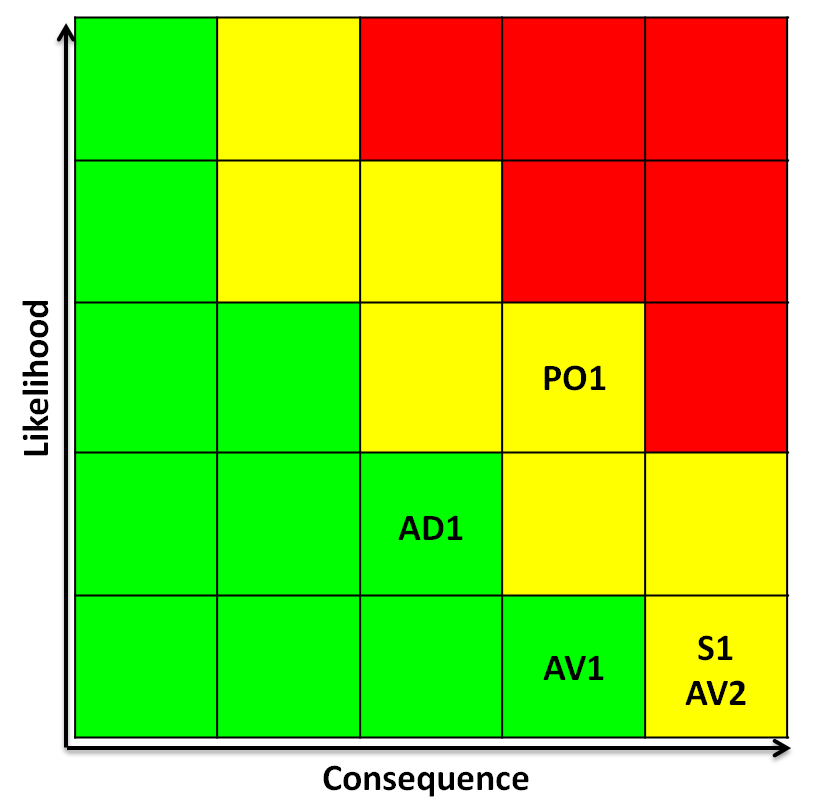
\includegraphics[width=4in]{images/conclusion_1.png}
\caption{Systems level risk chart.}
\label{fig:risk_chart}
\end{figure}

Two risks exist regarding the Avionics subsystem.  The higher priority risk of two (AV2) is a low likelihood, high consequence risk that the Avionics system will not be capable of providing the required latency for ADCS and the Payload subsystem.  The second risk (AV1) is a low likelihood, medium consequence risk that the Avionics subsystem will not be capable of processing all of the incoming data.  

Finally, there is a low consequence, low likelihood risk (AD1) that ADCS will exceed the system mass budget.  A trade between mass and power was carried out in the design of the torque coils since both the mass and power budgets of the system are tight.  Additionally, in this stage of the design, the system components and properties still have the potential to change.  Therefore, if the torque coil design needs to be altered in order to reduce the power draw of the system, the mass might increase to be over the maximum set by the CubeSat standards for a 3U Cubesat.  However, this is a low consequence, low likelihood risk since currently the system mass with margin is under the maximum.

		\subsection{Future Work}\label{sec:conclustions_futurework}
More iterations in the design process need to be carried out before the design can be completed.  Discussed below, in priority order, is future work for the DeMi system:
\begin{itemize}
\item A more detailed model of the temperature dependence of battery and solar panel performance needs to be developed in order to more accurately calculate the power that can be supplied to the system.  
\item A more detailed model of the temperature gradient across the satellite needs to be developed in order to determine whether the proposed heating design will be effective.  
\item A more accurate model of external disturbances and an attitude control loop need to be developed by ADCS.
\item More research and analysis needs to be carried out regarding the interface with Payload, and it must be confirmed that the Avionics system can process all information at the required speed.  
\item As the design continues to mature, the structural model will need to continue to be updated with new parts and part positions in order to ensure that the system continues to meet CubeSat design standards.
\item It must be verified that the structure and components will survive the launch environment.
\item Further research needs to be conducted on the construction and use of the measuring tape antenna.  
\end{itemize}

		
		%%%%%%%%%%%%%%%%%%%%%%%%%%%%%%%%%%%%%%%%%%%%%%%%%%%%%%%%%%%%%%%%%%%%%%%%%%%%%%%%%%%%%%%%%%%%%%%%%%%%%%%%%%%%%%%%%%%%%%%%%%%%%%%%%%%%%%%%%%%%%%%%%%%%%%%%
\FloatBarrier
\newpage

\section{Acknowledgment - AC, ZG}
The authors would like to thank K. Cahoy, J. Hoffman, A. Golkar, J. Craig, J. Connor, and F. Alibay for their guidance, instruction, and patience throughout the duration of the project.

A special thanks goes to I. Harris, H. Hemmati, S. Unwin, E. Deems, D. Seal and M. Ingham for their contributions to the preliminary design review and final design document.

The authors are grateful to A. Marinan, K. Kingsbury, M. Weber, C. Kerr, B. Novak, K. McLaughlin, J. Pinheiro, P. Dave, and W. Lohmeyer for useful discussions and conversations about specific subsystems.	
	
%%%%%%%%%%%%%%%%%%%%%%%%%%%%%%%%%%%%%%%%%%%%%%%%%%%%%%
% APPENDICES
\FloatBarrier
\newpage
\appendix
\section{Requirements} \label{app:requirements}

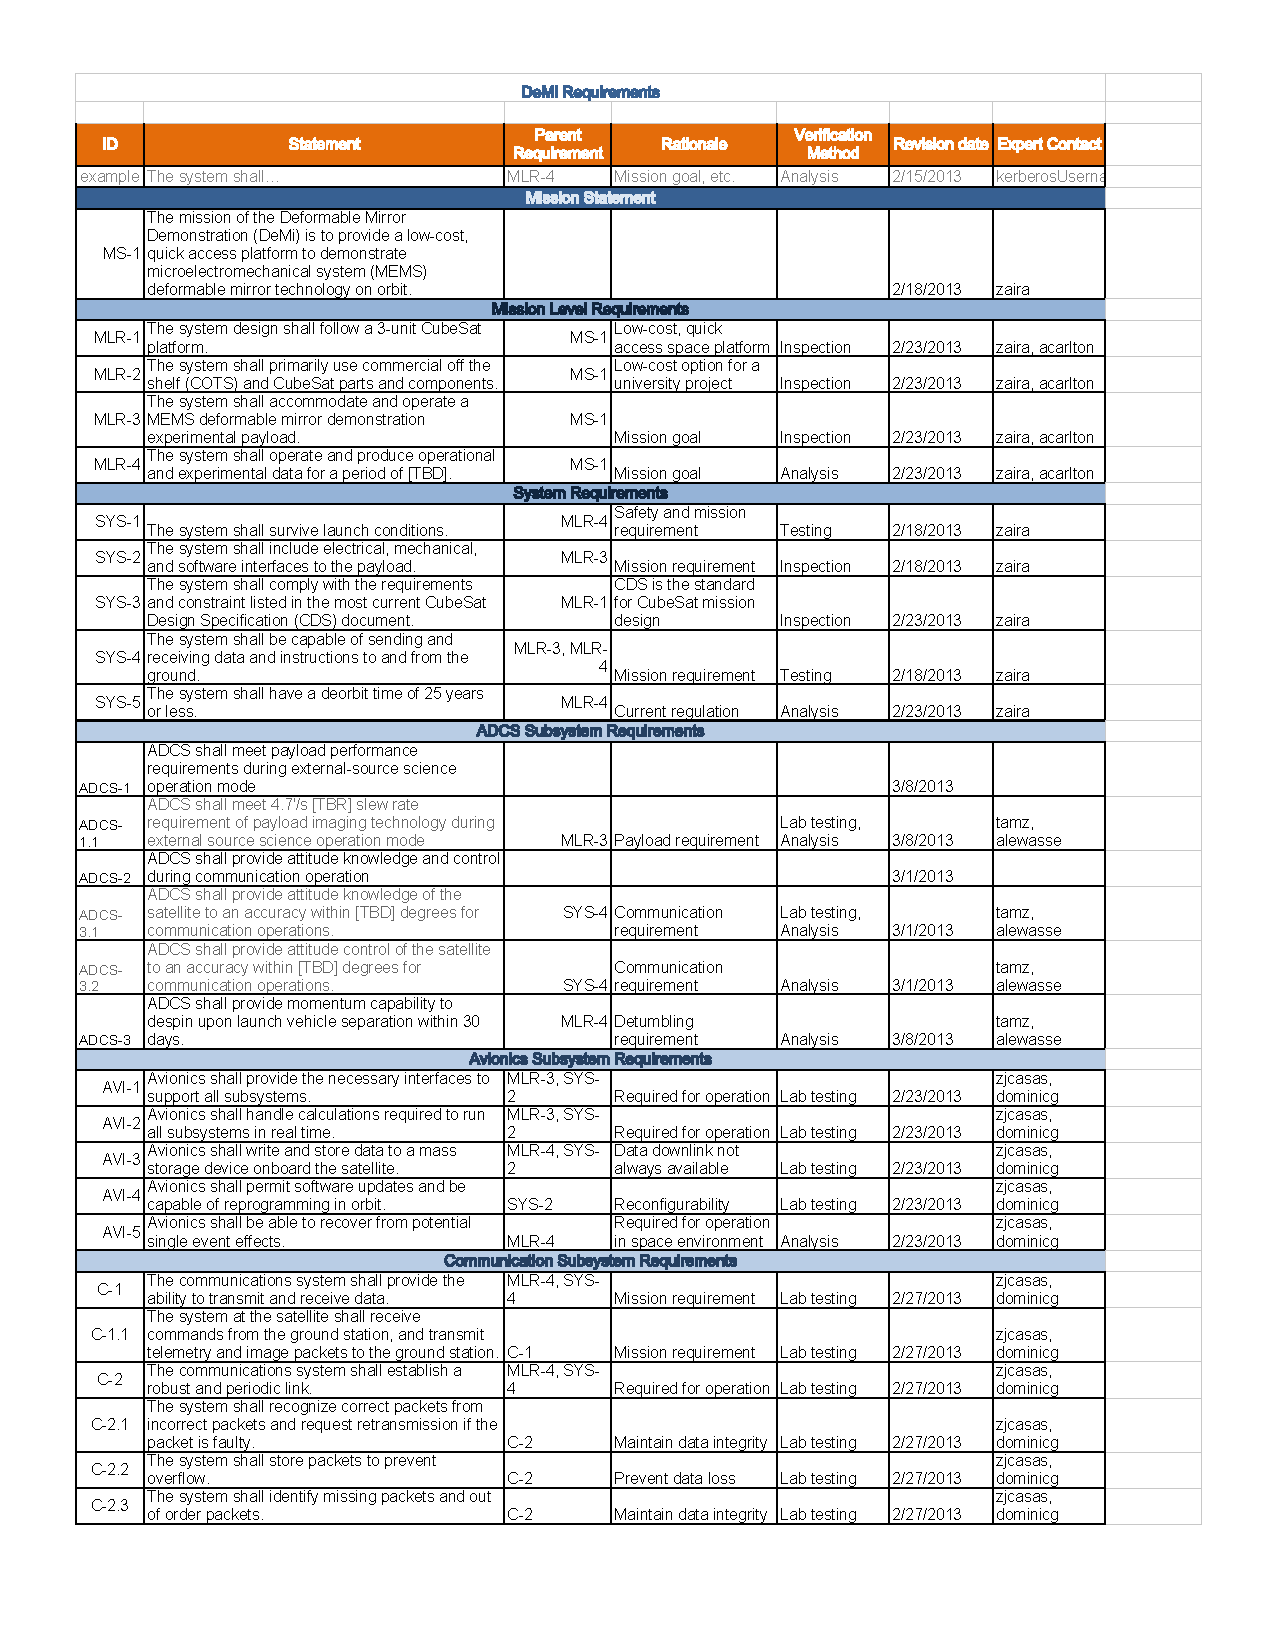
\includepdf[pages={-}]{images/Requirements.pdf}

\newpage

\begin{landscape}
\section{Payload Components} \label{app:payload_components}
\small
\begin{center}
\begin{longtable}{| p{3.25cm} | p{2.2cm} | p{3cm} | p{1.75cm} | p{2.5cm} | p{1.55cm} | p{5cm} |}
\hline
    \textbf{Assembly} & \textbf{Specific components} & \textbf{Description} & \textbf{Mass (g) - to 0.01} & \textbf{Additional Notes about Mass} & \textbf{Intensity transmission (\%)} &  \\ \hline 
    \midrule 
    \multirow{5}{*}{\parbox{3.25cm}{Aperture Lens}} & LA4647-A & lens  & 20    &       & 99.5  & Reflectivity over coating avg $<$ 0.5\% \\ 
          & LMR05 & housing & 1.75  &       &       &  \\
          & MSA8  & adapter for post & 0.55  &       &       &  \\
          & MS05R & miniseries post & 2.43  &       &       &  \\
          & base  & machined & 11.43 & ESTIMATED$^1$ &       &  \\ \hline
    \multirow{6}{*}{\parbox{3.25cm}{Collimating Lens}} & A375TM-A & mounted asphere & 0.2   &       & 99.5  & Reflectivity over coating avg $<$ 0.5\% \\ 
          & S05TM09 & adapter & 1.4   &       &       &  \\
          & LMR05 & housing & 1.75  &       &       &  \\
          & MSA8  & adapter for post & 0.55  &       &       &  \\
          & MS05R & miniseries post & 2.43  &       &       &  \\
          & base  & machined & 11.43 & ESTIMATED$^1$&       &  \\ \hline
    \multirow{5}{*}{\parbox{3.25cm}{Polarizer for external source}} & LPVISB050 & mounted linear polarizer & 1.39  &       & 50    & Polarizer \\ 
          & LMR05 & housing & 1.75  &       & 99.99 & Extinction ratio: $>$ 10,000:1 \\
          & MSA8  & adapter for post & 0.55  &       &       &  \\
          & MS05R & miniseries post & 2.43  &       &       &  \\
          & base  & machined & 11.43 & ESTIMATED$^1$ &       &  \\ \hline
    \multirow{5}{*}{Laser} & CPS186 & laser & 1.9   &       &       &  \\ 
          & AD8F  & adapter & 4.36  &       &       &  \\
          & LMR1  & housing & 3.78  &       &       &  \\
          & MSA8  & adapter for post & 0.55  &       &       &  \\
          & MS05R & miniseries post & 2.43  &       &       &  \\
          & base  & machined & 11.43 & ESTIMATED$^1$  &       &  \\ \hline
    \multirow{6}{*}{\parbox{3.25cm}{Polarizer for Laser}} & GT5-A & mounted Glan-Taylor polarizer & 1.15  &       & 50    & Polarizer \\ 
          & SM05PM5 & adapter & 3.04  &       & 99    & Reflectivity over coating avg $<$ 1\% \\
          & LMR05 & housing & 1.75  &       & 99.999 & Extinction ratio: $>$ 100,000:1 \\
          & MSA8  & adapter for post & 0.55  &       &       &  \\
          & MS05R & miniseries post & 2.43  &       &       &  \\
          & base  & machined & 11.43 & ESTIMATED$^1$ &       &  \\ \hline
    \multirow{5}{*}{Flat Mirror} & PF05-03-P01 & mirror & 0.76  &       & 97.5  & Reflectivity over coating avg $>$ 97.5\% \\ 
          & LMR05 & housing & 1.75  &       &       &  \\
          & MSA8  & adapter for post & 0.55  &       &       &  \\
          & MS05R & miniseries post & 2.43  &       &       &  \\
          & base  & machined & 11.43 & ESTIMATED$^1$ &       &  \\ \hline
    \multirow{6}{*}{\parbox{3.25cm}{Beamsplitter for Sources}} & 05FC16PB.5 & beamsplitting cube & 5.03  & ESTIMATED from glass cube (Newport) & 90 or 99.5 & R\_P $>$ 90\%, R\_S $>$ 99.5\% \\ 
          & UPH-CH.5 & BS housing & 2.43  &       & 99.8  & Extinction Ratio: $>$ 500:1 \\
          & U50-A & aperture mount & 4.29  &       &       &  \\
          & MSA8  & adapter for post & 0.55  &       &       &  \\
          & MS05R & miniseries post & 2.43  &       &       &  \\
          & base  & machined & 11.43 & ESTIMATED$^1$ &       &  \\ \hline
    \multirow{6}{*}{\parbox{3.25cm}{Beamsplitter for Mirrors}} & 05FC16PB.5 & beamsplitting cube & 5.03  &       & 90 or 99.5 & $R_P$ $>$ 90\%, $R_S$ $>$ 99.5\% \\ 
          & UPH-CH.5 & BS housing & 2.43  &       & 99.8  & Extinction Ratio: $>$ 500:1 \\
          & U50-A & aperture mount & 4.29  &       &       &  \\
          & MSA8  & adapter for post & 0.55  &       &       &  \\
          & MS05R & miniseries post & 2.43  &       &       &  \\
          & base  & machined & 11.43 & ESTIMATED$^1$ &       &  \\ \hline
    \multirow{5}{*}{\parbox{3.25cm}{Quarter Waveplate}} & WPQ05M-670 & waveplate & 6.67  &       & 99.5  & Reflectance per surface $<$ 0.25\% \\ 
          & LMR05 & housing & 1.75  &       &       &  \\
          & MSA8  & adapter for post & 0.55  &       &       &  \\
          & MS05R & miniseries post & 2.43  &       &       &  \\
          & base  & machined & 11.43 & ESTIMATED$^1$ &       &  \\ \hline
    \multirow{4}{*}{\parbox{3.25cm}{Deformable Mirror System}} & DMs   & BMC   & 73.71 & only 2 sig figs & 99    & Reflectance $>$ 99\% \\ 
          & Driver &       & 93.55 & only 2 sig figs &       &  \\
          & post (if nec.) & machined & 7.38  & ESTIMATED from RS05P (upper est.) &       &  \\
          & base  & machined & 15.26 & ESTIMATED from BE1+CF125 (upper est.) &       &  \\ \hline
    Shack-Hartmann Lenslet & MLA150-5C-M & micro lenslet array & 2     & will go inside lens tube of detector & 75    & Reflectivity $<$ 25\% (includes chrome mask) \\ \hline
    \multirow{3}{*}{Detector} & UI-5241LE-M & CMOS  & 24    &       & 46.64 &  \\ 
          & post  & machined & 7.38  & ESTIMATED from RS05P (upper est.) &       &  \\
          & base  & machined & 15.26 & ESTIMATED from BE1+CF125 (upper est.) &       &  \\ \hline
    Optical Platform/Breadboard &       & machined & 250   & ESTIMATED &       &  \\ \hline
    Optical Enclosure &       &       & 300   & ESTIMATED from XE25C1\_M (upper est.) &       &  \\ \hline
    TOTAL MASS &       &       & 996.88 &       &       &  \\
    Mass with 25\% margin &       &       & 1246.1 &       &       &  \\ \hline
\hline
\end{longtable}
$^1$Estimated from ThorLabs miniseries post MS075.
\end{center}
\end{landscape}

\clearpage



\section{Link Budgets} \label{app:link_budgets}
\textbf{Uplink Budget}
\small
\begin{center}
\begin{longtable}{| p{3.9cm} | p{1.6cm} | p{1.4cm} | p{1.4cm} | p{1.4cm} | p{5cm} |}
\hline
    \textbf{Item}  & \textbf{Symbol} & \textbf{Units}  & \textbf{Worst Case} & \textbf{Best Case} & \textbf{Source}  \\
    \hline \hline
    frequency & $f$     & GHz   & 0.45  & 0.45  & Hardware \\ \hline
    wavelength & $\lambda$ & m     & 0.667 & 0.667 & Lambda=c/f \\ \hline
    propagation path length & $r$     & km    & 2082  & 500   & Mission/ ITU-R P.676-9 eq 17, 18, 19 \\\hline
    data rate & $R$     & bps   & 19200 & 19200 & Hardware \\\hline
    data rate & $R$     & dB    & 42.833 & 42.833 &  \\\hline
    transmit antenna diameter & $D_t$  & m     & 18.29 & 18.29 & Wallops \\\hline
    transmit antenna beam width & $\theta_t$ & deg   & 2.9   & 2.9   & Wallops \\\hline
    transmitter power & $P$     & W     & 1     & 2     & from DICE mission \\\hline
    transmitter power & $P$     & dBW   & 0     & 3.01  &  \\\hline
    transmit antenna gain & $G_t$  & dBi   & 35    & 35    & Wallops \\\hline
    transmit antenna pointing offset & $e_t$  & deg   & 1     & 0     &  \\\hline
    transmit antenna pointing loss & $L_{pt}$ & dB    & 1.5   & 0     & Antenna Gain Pattern \\\hline
    transmitter line loss & $L_l$  & dBW   & 1     & 0.5   & Line Loss for Coax Cable \cite{loss-calc} \\\hline
    equivalent isotropic radiated power & $EIRP$  & dbW   & 32.5  & 37.51 & SMAD 16-20 \\\hline
    receive antenna efficiency & $\eta$   &       & 0.5   & 0.5   & approximate efficiency \\\hline
    receive antenna beam width & $\theta_r$ & deg   & 65    & 65    & Antenna Gain pattern \\\hline
    receive antenna gain & $G_r$  & dBi   & -4    & 3     &  \\\hline
    receive antenna pointing offset & $e_r$  & deg   & 5     & 1     & SMAD \\\hline
    receive antenna pointing loss & $L_{pr}$ & dB    & 3     & 0     &  \\\hline
    space loss & $L_s$  & dB    & 151.884 & 139.494 & SMAD 16-22 \\\hline
    Dry-air and water vapor loss & $L_{atm}$ & dB    & 0.02  & 0.02  & ITU-R P.676-9 Figure 6 \\\hline
    total loss & $L_{comb}$ & dB    & 157.404 & 140.014 &  \\\hline
    Sky Temperature & $T_{sky}$ & K     & 60    & 30    &  \\\hline
    Ground Temperature & $T_{ground}$ & K     & 290   & 290   &  \\\hline
    Antenna Temperature & $T_{antenna}$ & K     & 117.5 & 95    & Pozar Eq \\\hline
    Receiver Temperature & $T_{receiver}$ & K     & 3270  & 3270  & Hardware \\\hline
    System Noise Temperature & $T_s$  & K     & 3387.5 & 3365  & Pozar Eq \\\hline
    System Noise Temperature & $T_s$  & dB    & 35.299 & 35.27 &  \\\hline
    receiver G/T & --    & dB    & -39.299 & -32.27 & SMAD 16-27 \\\hline
    Boltzmann constant & $k_b$  & dB    & -228.599 & -228.599 & -- \\\hline
    C/N0  & --    & dB    & 64.397 & 93.826 & SMAD 16-30 \\\hline
    Eb/N0 & --    & dB    & 21.563 & 50.993 & SMAD 16-31 \\\hline
    Bit Error Rate & $BER$   & \%    & 10\^-5 & 10\^-5 &  \\\hline
    Required Eb/N0 & --    & dB    & 9.5   & 9.5   & SMAD figure 16-16 \\\hline
    margin & --    & dB    & 12.064 & 41.493 & SMAD16-33 \\
\hline
\end{longtable}
\end{center}


\newpage

\textbf{Downlink Budget}
\small
\begin{center}
\begin{longtable}{| p{3.9cm} | p{1.6cm} | p{1.4cm} | p{1.4cm} | p{1.4cm} | p{5cm} |}
\hline
    \textbf{Item}  & \textbf{Symbol} & \textbf{Units}  & \textbf{Worst Case} & \textbf{Best Case} & \textbf{Source}  \\
    \hline \hline
    frequency & $f$     & GHz   & 0.465 & 0.465 & Hardware \\\hline
    wavelength & $\lambda$ & m     & 0.645 & 0.645 & Lambda=c/f \\\hline
    propagation path length & $r$     & km    & 2082  & 500   & Mission/ITU-R P.676-9 eq 17, 18, 19 \\\hline
    data rate & $R$     & bps   & 1500000 & 1500000 & Hardware \\\hline
    data rate & $R$     & dB    & 61.761 & 61.761 &  \\\hline
    transmit antenna length & $l$     & m     & 0.164 & 0.164 & quarter-wave monopole \\\hline
    transmit antenna beam width & $\theta_t$ & deg   & 65    & 65    & Antenna Gain Pattern \\\hline
    transmitter power & $P$     & W     & 1     & 2     & from DICE mission \\\hline
    transmitter power & $P$     & dBW   & 0     & 3.01  &  \\\hline
    transmit antenna gain & $G_t$  & dBi   & -4    & 3     &  \\\hline
    transmit antenna pointing offset & $e_t$  & deg   & 5     & 1     & SMAD \\\hline
    transmit antenna pointing loss & $L_{pt}$ & dB    & 3     & 0     &  \\\hline
    transmitter line loss & $L_l$  & dBW   & -1    & -0.8  & Line Loss for Coax Cable \cite{loss-calc} \\\hline
    equivalent isotropic radiated power & $EIRP$  & dbW   & -6    & 6.81  & SMAD 16-20 \\\hline
    receive antenna efficiency & $\eta$   & --    & 0.5   & 0.5   & approximate efficiency \\\hline
    receive antenna beam width & $\theta_r$ & deg   & 2.9   & 2.9   & Wallops \\\hline
    receive antenna gain & $G_r$  & dBi   & 35    & 35    & Wallops \\\hline
    receive antenna pointing offset & $e_r$  & deg   & 1     & 0     &  \\\hline
    receive antenna pointing loss & $L_{pr}$ & dB    & 1.5   & 0     & Antenna Gain pattern \\\hline
    space loss & $L_s$  & dB    & 152.169 & 139.778 & SMAD 16-22 \\\hline
    Dry-air and water vapor loss & $L_{atm}$ & dB    & 0.02  & 0.02  & ITU-R P.676-9 Figure 6 \\\hline
    total loss & $L_{comb}$ & dB    & 155.689 & 138.998 &  \\\hline
    Sky Temperature & $T_{sky}$ & K     & 290   & 290   &  \\\hline
    Ground Temperature & $T_{ground}$ & K     & 60    & 30    &  \\\hline
    Antenna Temperature & $T_{antenna}$ & K     & 232.5 & 225   & Pozar Eq \\\hline
    Receiver Temperature & $T_{receiver}$ & K     & 66    & 66    & Wallops \\\hline
    System Noise Temperature & $T_s$  & K     & 298.5 & 291   & Pozar Eq \\\hline
    System Noise Temperature & $T_s$  & dB    & 24.749 & 24.639 &  \\\hline
    receiver G/T & --    & dB    & 10.251 & 10.361 & SMAD 16-27 \\\hline
    Boltzmann constant & $k_b$  & dB    & -228.599 & -228.599 &  \\\hline
    C/N0  & --    & dB    & 77.161 & 106.772 & SMAD 16-30 \\\hline
    Eb/N0 & --    & dB    & 15.4  & 45.011 & SMAD 16-31 \\\hline
    Bit Error Rate & $BER$   & \%    & 10\^-5 & 10\^-5 &  \\\hline
    Required Eb/N0 & --    & dB    & 9.5   & 9.5   & SMAD figure 16-16 \\\hline
    margin & --    & dB    & 5.9   & 35.511 & SMAD 16-33 \\
\hline
\end{longtable}
\end{center}

\noindent
\newline
\newpage


%%%%%%%%%%%%%%%%%%%%%%%%%%%%%%%%%%%%%%%%%%%%%%%%%%%%%%
% REFERENCES
\begin{thebibliography}{9}

%%%%%%%%%%%%%%%%%%%%%%%%%%%%%%%%%%%%%%%%%%%%%%%%%%%%%%
% REFERENCES


%%% OVERVIEW

\bibitem{bos-micro-demi}
“Mini-DM.” (2012) URL \url{http://www.bostonmicromachines.com/light-modulator.htm}. (visited April 30, 2013).

\bibitem{cahoy-unpublished}
Cahoy, K., A. Marinan, C. Kerr, K. Cheng, S. Jamil, “CubeSat deformable mirror demonstration,”.In SPIE Conference on Space Telescopes and Instrumentation 2012: Optical, Infrared, and Millimeter Wave. Amsterdam, Netherlands,2012.

\bibitem{adaptive-optics-overview}
“Adaptive Optics Overview.” (2012) URL \url{http://www.irisao.com/technology.html}. (visited April 30, 2013).

\bibitem{serabyn2010}
Serabyn, E., Mawet, D., \& Burruss, R., ``An image of an exoplanets separated by two diffraction beamwidths from a star''. Nature, Vol. 464, 2010, pp. 1018-1020.

\bibitem{cubesat-specs}
CubeSat Design Specifications, California Polytechnic State University, \url{http://www.cubesat.org/index.php/documents/developers}

\bibitem{nasa-deorbit}
NASA-STD-8719.14, \url{http://www.hq.nasa.gov/office/codeq/doctree/871914.pdf}
%% Misison Overview
\bibitem{mission_cubesat}
Munakata R., \emph{CubeSat Design Specification Rev. 12}, The CubeSat Program, CalPoly State Univ., San Luis Obispo, CA, 2009.

\bibitem{mission_deorbit}
\emph{Process for Limiting Orbital Debris}. NASA-STD-8719.14A, 2011, p. 21. URL http://www.hq.nasa.gov/office/codeq/doctree/871914.pdf (visited May 13, 2013)

\bibitem{mission_aiaa}
\emph{Mass Properties Control for Space Systems (S-120-2006)}, American Institute of Aeronautics and Astronautics, Reston, 2006.

%%% PAYLOAD

\bibitem{FGadaptiveoptics}
   Tyson, Robert K. and Benjamin W. Frazier. 
   \emph{Field Guide to Adaptive Optics}. Bellingham, WA: SPIE Press,
   2012.  Internet resource.

\bibitem{gerchberg}
   Kay J., Kasdin, N. J., Belikov, R.
   \emph{Wavefront correction in a shaped-pupil coronagraph using a Gerchberg-Saxton-based estimation scheme}, Astronomical Adaptive Optics Systems and Applications III, Vol. 6691, SPIE Proceedings, Washington, D.C., 2007.

\bibitem{cahoy2013}
   Cahoy, K. L., A. Marinan, B. Novak, C. Kerr, M. Webber. 
   \emph{Wavefront control in space with MEMS deformable mirrors},
   Photonics West, MEMS Adaptive Optics VII, Vol. 8617, SPIE,
   Washington, D.C., 2013.

\bibitem{radiation_optics}
   Nicoletta, C. A. and A. G. Eubanks.
   \emph{Effect of Simulated Space Radiation On Selected Optical
     Materials}. Washington, D.C.: National Aeronautics and Space
   Administration, 1972.

\bibitem{traeger}
   Traeger, F., \emph{Springer Handbook of Lasers and Optics}. New
   York: Springer, 2007.

\bibitem{demtroeder}
   Demtroeder, W.
   \emph{Laser Spectroscopy: Basic Concepts and Instrumentation}, 3rd
   ed. Berlin: Spring-Verlag, 2003.

\bibitem{newport_nanopositioner}
   NPX NanoPositioning Linear Stages, Newport Corporation,
   URL \url{http://www.newport.com/NPX-Series-NanoPositioning-Linear-Stages/843084/1033/info.aspx}
   (visited May 10, 2013).

\bibitem{centroids}
Thomas, S., et al. "Comparison of centroid computation algorithms in a Shack-Hartmann sensor". \emph{Monthly Notices of the Royal Astronomical Society}, MN-06-0231-MJ.R1, 2006.

\bibitem{ctio_AO}
   Tokovinin, A., (May 28, 2001). ``Adaptive optics tutorial at CTIO'' URL
   \url{http://www.ctio.noao.edu/~atokovin/tutorial/part3/wfs.html}, 
   (visited 10 May 2013).

\bibitem{MLA150}
   MLA150-5C, ThorLabs Inc.,
   URL \url{http://thorlabs.com/thorProduct.cfm?partNumber=MLA150-5C}
   (visited 5 May 2013).

\bibitem{BMC}
Boston Micromachines Corporation, <http://www.bostonmicromachines.com/light-modulator.htm> (accessed 5 May 2013).

\bibitem{zemax}
   ZEMAX, Software Package, Ver. 13, Radiant Zemax LLC, Redmond, WA, 2013.

\bibitem{correia2010}
  Correia, C., H.-F. Raynaud, C. Kulcsar, J.-M. Conan, "On the optimal reconstruction and control of adaptive optical systems with mirror dynamics," JOSA A, 27(2), 333-349, doi:10.1364/JOSAA.27.000333 (2010).

\bibitem {greivenkamp}
   Greivenkamp, John E. 
   \emph{Field Guide to Geometrical Optics}, Bellingham, WA: SPIE, 2004. Print.


%%% POWER

\bibitem{CS-image}
Image from Clyde Space.  URL \url{http://www.clyde-space.com/cubesat_shop/solar_panels_-_deployable}, (visited May 05, 2013).

\bibitem{libertad-1} (2012).  ``CubeSat Kit -- In Space.''  URL \url{http://www.cubesatkit.com/content/space.html}, (visited May 05, 2013).

\bibitem{EPS-manual} Strain, A, (February 14, 2011).  ``User Manual: CubeSat 3U Electronic Power System.'' URL \url{http://www.clyde-space.com/documents/2471}, (visited May 05, 2013).

\bibitem{PDM-manual} Worrall, K, (March 14, 2011).  ``CubeSat Power Distribution Module User Manual.'' URL \url{http://www.clyde-space.com/documents/2560}, (visited May 05, 2013).

\bibitem{Battery-manual} McLaren, V, (April 28 2010).  ``User Manual: Standalone 30Wh Battery.''  URL \url{http://www.clyde-space.com/documents/1902}, (visited May 05, 2013).

\bibitem{Solar-panel-datasheet} (March 16 2012). ``CubeSat Solar Panels.''  URL \url{http://www.clyde-space.com/documents/2625}, (visited May 05, 2013).

%%% COMMUNICATIONS

\bibitem{ITU-R}
``ITU-R P.676-9'', URL \url{http://www.itu.int/dms_pubrec/itu-r/rec/p/R-REC-P.676-9-201202-I!!PDF-E.pdf}, (visited April 2013).

\bibitem{pozar}
Pozar, David M., \emph{Microwave and RF Design of Wireless Systems}, Wiley, New York City, NY, 2001.


%%% AVIONICS

\bibitem{avionics_clyde_space}
Clyde Space. CubeSat Shop. URL \url{http://www.clyde-space.com/cubesat_shop/obdh/364_mission-interface-computer-grande-em}, visited May 5, 2013. 

\bibitem{avionics_FPGA}
T. Saegusa, T. Maruyama, Y.Yamaguchi, "How fast is an FPGA in image processing?", FPL 2008, pp. 77 – 82.

\bibitem{avionics_RTOS}
URL \url{http://www.freertos.org/RTOS.html} (visited May 14, 2013).

\bibitem{avionics_pumpkin}
URL \url{http://www.pumpkininc.com/content/doc/press/salvoflyer.pdf} (visited May 14, 2013).


%%% ADCS
\bibitem{adcs_survey}
Sofyali, A. and Aslan, A.R. \emph{Magnetic Attitude Control of Small Satellites: A Survey of Applications and A Domestic Example}. Istanbul Technical University. Istanbul, Turkey. 

\bibitem{adcs_smad1}
Wertz, James, \emph{Space Mission Engineering: The New SMAD}, Microcosm Press, Hawthorne, CA, 2011. pp. 578. 

\bibitem{adcs_smad2}
Wertz, James, \emph{Space Mission Engineering: The New SMAD}, Microcosm Press, Hawthorne, CA, 2011. pp. 570-573. 

\bibitem{adcs_compass}
Aydinlioglu, A. and Hammer, M. \emph{COMPASS-1 Picosatellite: Magnetic Coils for Attitude Control}. University of Applied Sciences Aachen, Aachen, Germany. 

\bibitem{adcs_ion}
Gregory, S. \emph{Attitude Control System Design for ION, the Illinois Observing Satellite}. Urbana, Illinois, 2004.
%%% THERMAL

\bibitem{satnews}
\url{http://www.satnews.com/images_upload/604251372/CubeSat_UKSA.jpg}

\bibitem{minco}
\url{http://ektron.minco.com/uploadedImages/Products/foilheater.jpg}

\bibitem{ids-imaging}
\url{http://en.ids-imaging.com/}

\bibitem{omega}
\url{http://www.omega.com/Temperature/pdf/44000_THERMIS_ELEMENTS.pdf}

%%% STRUCTURES

\bibitem{cubesatkit} %[1]
\url{http://www.cubesatkit.com/content/design.html}

\bibitem{cubesatshop} %[2]
\url{http://www.cubesatshop.com/index.php?page=shop.product_details&category_id=6&flypage=flypage.tpl&product_id=66&option=com_virtuemart&Itemid=70&vmcchk=1&Itemid=70}

\bibitem{isis-image} %[3]
\url{http://www.isispace.nl/brochures/ISIS_AntS_Brochure_v.7.11.pdf}

\bibitem{uhf-cubesat} %[4]
Tamamoto, M., W. Shiroma. \emph{Active Antennas and UHF Antennas for CubeSat Applications}, Honolulu, HI, 2002, page 101.

\bibitem{cubesat-leo} %[5]
Waydo, S., D. Henry, M. Campbell. \emph{CubeSat Design for LEO-Based Earth Science Missions, Seattle, WA, 2001}, page 8.


%%% CONCLUSION
\bibitem{ION-mission}
Gregory, S. \emph{Attitude Control System Design for ION, the Illinois Observing Satellite}. Urbana, Illinois, 2004. 

%%% Appendices
\bibitem{loss-calc}
Amateur Radio Repeater Geezers, \emph{Types of Coax Cable and Line Loss Calculator}, URL \url{http://www.arrg.us/pages/Loss-Calc.htm}, (visited May 5, 2013).

%%% TO BE SORTED


%\bibitem{kim00}
   %Kim. (2000).
  %\emph{\ Simulation Study of A Low-Low Satellite-to-Satellite Tracking Mission}. (Doctoral dissertation)
  %The University of Texas at Austin, TX.



\bibitem{SMAD}
Wertz, James, \emph{Space Mission Engineering: The New SMAD}, Microcosm Press, Hawthorne, CA, 2011.


\end{thebibliography}

\end{document}


